


\section*{Learning Objectives}
\begin{itemize}
\item Introduce material that is commonly included in a second or third year Linear Algebra Course
\item Provide a resource for use after you leave ROB 101.
\end{itemize}

\section*{Outcomes}
\begin{itemize}
%\item Hyperplanes and an Interesting Example
\item Complex numbers obey the same rules of arithmetic as the real numbers, if you really understand the real numbers!
\item Eigenvalues and eigenvectors of square matrices
\item Symmetric matrices have real eigenvalues and admit orthonormal eigenvectors 
\item Positive definite matrices allow one to generalize the Euclidean norm
\item The Singular Value Decomposition (SVD) allows one to quantify the degree to which vectors are linearly independent. This is super useful in engineering practice.
\item Matrices are good for other things than representing systems of equations: they also allow one to transform vectors in interesting ways, giving rise to the concept of \textit{linear transformations}.
\item Many more facts about basis vectors.
\end{itemize}


\vspace*{1.5cm}





\newpage


\section{Complex Numbers and Complex Vectors}
\label{sec:ComplexNumbers}

Here are some video resources that you may enjoy consulting:

\begin{itemize} 

\item \url{https://youtu.be/T647CGsuOVU}

\item \url{https://youtu.be/2HrSG0fdxLY}

\item \url{https://youtu.be/N9QOLrfcKNc}

\item \url{https://youtu.be/DThAoT3q2V4}

\item \url{https://youtu.be/65wYmy8Pf-Y}

\end{itemize}

The story of complex numbers begins with the quadratic equation $x^2 + 1=0$, which has no real solutions! After much soul searching, the mathematics community finally embraced the notion of an \textbf{imaginary quantity} $\im$ defined by
\begin{equation}
    \label{eq:ImaginaryQuanity}
    (\im)^2:= -1. 
\end{equation}
More commonly, we write this as 
\begin{equation}
    \label{eq:ImaginaryQuanity02}
    \im= \sqrt{-1}. 
\end{equation}
The set of \textbf{complex numbers} is then defined as 
\begin{equation}
    \label{eq:ComlexNumbers}
    \cp:=\left\{x + \im~ y~| x\in \real, y \in \real \right\}. 
\end{equation}
If $z=x+ \im~ y \in \cp$, then we define
\begin{equation}
    \label{eq:RealImagParts}
    \begin{aligned}
    x&:= \repart{z}~~\text{the {\bf real part} of}~~z\\
    y&:= \impart{z}~~\text{the {\bf imaginary part} of}~~z.
    \end{aligned}
\end{equation}
We note that both $x$ and $y$ are real numbers. Complex numbers of the form $0 + \im~y$ are called \textbf{imaginary numbers}. We view a \textbf{real number} $x\in \real$ as being a complex number of the form $x + \im~0$. In other words, we view $\real \subset \cp.$ In addition, we define the \textbf{complex conjugate} of $z=x+\im~y$ to be
\begin{equation}
    \label{eq:complexConjugate}
z^\ast:= x - \im~y,
\end{equation}
that is, $\impart{z^\ast} = - \impart{z}$, while $\repart{z^\ast}=\repart{z}$.
\vspace*{0.2cm}


\begin{figure}[htb!]
\centering
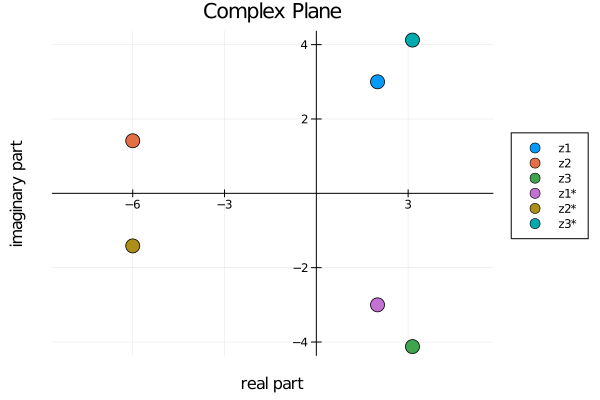
\includegraphics[width=0.6\textwidth]{graphicsAppendices/CoolThings/ComplexPlane.png}
\caption[]{The complex plane has $x$-axis given by the real part of a complex number and $y$-axis given by the imaginary part of a complex number. Here, we plot $z_1, z_2, z_3$ from Example~\ref{ex:ComplexNumbers} and their complex conjugates. }
\label{fig:ComplexPlane}
\end{figure}

\vspace*{0.2cm}
\begin{example}
\label{ex:ComplexNumbers}
For the following are complex numbers, compute their real and imaginary parts as well as their complex conjugates. Also, plot them in the complex plane.
$$\begin{aligned}
z_1 &= 2 + \im~3\\
z_2&= -6 + \im~ \sqrt{2} \\
z_3&= \pi -\im~\sqrt{17}.
\end{aligned}  $$
\end{example}

\textbf{Solution}

$$\begin{array}{lll}
\repart{z_1} = 2 & \impart{z_1} = 3 & z_1^\ast= 2 - \im~3\\
\repart{z_2} = -6 & \impart{z_2} = \sqrt{2} & z_2^\ast= -6 -\im ~\sqrt{2}\\
\repart{z_3} = 2\pi & \impart{z_3} = -\sqrt{17} & z_2^\ast= \pi + \im~ \sqrt{17}.\\
\end{array}  $$
All of these values are plotted in Fig.~\ref{fig:ComplexPlane}.


\Qed

\vspace*{0.2cm}

\subsection{Arithmetic of Complex Numbers: Enough to Get You By}

We'll define all of the major arithmetic operations. Just like operations with vectors and matrices, however, it's much more fun to do the calculations in Julia than by hand!\\

The \textbf{addition of two complex numbers} is defined by adding their respective real and imaginary parts, 
\begin{equation}
    \label{eq:AdditionComplexNumbers}
    \left(x_1 + \im~ y_1\right) + \left( x_2 + \im~ y_2 \right): = \left(x_1 + x_2 \right) + \im~ \left(y_1 + y_2  \right).
\end{equation}
This is very similar to how we add two vectors
$$\left[\begin{array}{c} x_1 \\ y_1 \end{array}  \right] + \left[\begin{array}{c} x_2 \\ y_2 \end{array}  \right] := \left[\begin{array}{c} x_1 + x_2\\ y_1 + y_2\end{array}  \right]$$
by adding their respective components. \\

The \textbf{multiplication} of two complex numbers is defined by
\begin{equation}
    \label{eq:MultiplicationComplexNumbers}
    \left(x_1 + \im~ y_1\right) \cdot \left( x_2 + \im~ y_2 \right): = \left(x_1 x_2 - y_1 y_2\right) + \im~ \left(x_1 y_2 + y_1 x_2 \right).
\end{equation}
This formula comes from applying basic algebra to the ``symbolic expression'' 
$$(a_1 + b_1) (a_2 + b_2) = a_1 a_2 + b_1 b_2 + a_1 b_2 + b_1 a_2 $$
and then substituting in
\begin{align*}
    a_1& := x_1\\
    a_2& := x_2\\
    b_1& := \im~y_1\\
    b_2& := \im ~y_2.
\end{align*}
The term $b_1 b_2 = (\im~y_1) \cdot (\im~y_2)= (\im)^2 y_1 y_2 = (-1) y_1 y_2$, which explains how the minus sign appears!\\

Let's note that if we multiply a complex number by its complex conjugate, then we obtain a real number. Indeed, 
\begin{equation}
    \label{eq:MultiplicationComplexNumbersByConjugate}
   z \cdot z^\ast =  \left(x + \im~ y\right) \cdot \left( x - \im~ y \right) = \left((x)(x) -(y)(-y) \right) + \im~ \left( (x) (-y) + (y)(x)  \right) = x^2 + y^2.
\end{equation}
The \textbf{magnitude of a complex number} $z=x+\im~y$ is denoted by $|z|$ and is defined by
\begin{equation}
    \label{eq:MagnitudeComplexNumbers}
   |z| := \sqrt{x^2 + y^2},
\end{equation}
or equivalently, by
\begin{equation}
    \label{eq:MagnitudeComplexNumbers02}
   |z| :=\sqrt{z \cdot z^\ast}.
\end{equation}
Both definitions are common and we note that the square root makes sense\footnote{Julia will recognize $\repart{z}^2 + \impart{z}^2$ as being a real number. It does not recognize $z \cdot z^\ast$ as a real number. In Julia, the command is ${\rm abs}(z)$, just as with a real number.} because the magnitude is a non-negative real number. \\

Using the complex conjugate, the \textbf{division of one complex number by another} can be defined, and subsequently, understood. We define 
\begin{equation}
    \label{eq:DivisionComplexNumbers}
    \frac {x_1 + \im~ y_1 }{x_2 + \im~ y_2 }: = \frac{\left(x_1 x_2 + y_1 y_2\right) +\im~\left(y_1 x_2 - x_1 y_2 \right)}{(x_2)^2 + (y_2)^2},
\end{equation}
and note that the denominator is real, and thus the indicated division can be treated as multiplication by one over the denominator. It follows that when $|z_2|\neq 0$, $z_1/z_2$ is a well-defined complex number. 
The formula \eqref{eq:DivisionComplexNumbers} is best understood from an alternative definition of complex division 
\begin{equation}
    \label{eq:DivisionComplexNumbers02}
   \frac{z_1}{z_2}:= \frac{z_1 \cdot z_2^\ast} {z_2 \cdot z_2^\ast} = \frac{z_1 \cdot z_2^\ast}{|z_2|^2}.
\end{equation}
Personally, we try to avoid using either one of these formulas and do the computations in Julia! Multiplication and division of complex numbers by hand is very error prone. For probably a century, engineering faculty have been torturing students by making them do such calculations by hand; at some point, it has to stop!\\

\vspace*{0.2cm}
\begin{example}
\label{ex:OperationsOnComplexNumbers}
For the following complex numbers, compute their sum, product, division, and magnitudes,
$$\begin{aligned}
z_1 &= 2 + \im~3\\
z_2&= -6 + \im~ \sqrt{2} \\
\end{aligned}  $$
\end{example}

\textbf{Solution}

$$ 
\begin{aligned}
z_1 + z_2 &= -4.0000+ \im4.4142  \\
z_1 \cdot z_2 &= -16.2426-\im15.1716 \\
\frac{z_1}{z_2} &=  -0.2041-\im 0.5481  \\
|z_1|&= 3.6056 \\
|z_2|&= 6.1644
\end{aligned}
$$
\Qed


\subsection{Angles of Complex Numbers and Euler's Formula: More Advanced Aspects}


\begin{figure}[htb!]
\centering
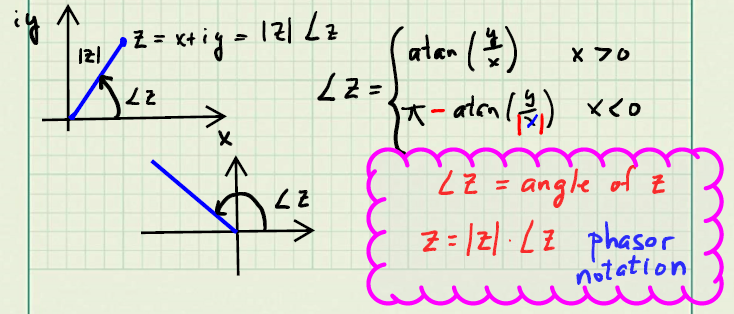
\includegraphics[width=0.8\textwidth]{graphicsAppendices/CoolThings/AngleComplexNumber.png}
\caption[]{It is often helpful to understand complex numbers as having a magnitude and an angle. This is similar to using polar coordinates in $\real^2$. Here, the angle of $z$ is denoted by $\angle z$ instead of $\theta$. Both conventions are common.}
\label{fig:ComplexPlaneTake2}
\end{figure}


For a pair of real numbers $(x,y)$, we were taught in High School how to express them in \textbf{polar coordinates} $(\rho, \theta)$, where 
\begin{equation}
    \label{eq:AnglePolarCoordinates}
    \begin{aligned}
    \rho &:=\sqrt{x^2 + y^2} \medskip \\
    \theta &:= \begin{cases} \arctan(y/x)& x > 0\\ \pi - \arctan( y/|x|) & x < 0\\
    {\rm sign}(y) ~\frac{\pi}{2} & x = 0, y\neq 0 \\
    \text{undefined} & x=0, y=0.\end{cases}
    \end{aligned}
\end{equation}

From polar coordinates $(\rho, \theta)$, we computed the \textbf{Cartesian Coordinates} $(x,y)$ as
\begin{equation}
    \label{eq:Polar2Cartesian}
    \begin{aligned}
    x&= \rho \cos(\theta)\\
    y&= \rho \sin(\theta).
    \end{aligned}
\end{equation}
Moving beyond High School, we can also express the above in terms of the canonical basis vectors $\{e_1, e_2 \}$ for $\real^2$ as
\begin{equation}
    \label{eq:Polar2Cartesian02}
\left[\begin{array}{c} x \\ y \end{array}  \right] = \rho \cos(\theta) e_1 +  \rho \sin(\theta) e_2.
\end{equation}
In fact, any (non-zero) vector $v\in \real^2$ can be expressed as 
\begin{equation}
    \label{eq:Polar2Cartesian03}
v = ||v|| \cos(\theta) e_1 +  ||v||\sin(\theta) e_2.
\end{equation}
Equation \eqref{eq:Polar2Cartesian03} hints at a natural way of expressing complex numbers.

\vspace*{0.5cm}
\begin{tcolorbox}[sharp corners, colback=green!30, colframe=green!80!blue, title=\textbf{\large Polar Coordinates Meet Complex Numbers and their Multiplication}]
For a non-zero complex number $z = x + \im~y$, we define its angle as in \eqref{eq:AnglePolarCoordinates}. Doing so allows us to express every (non-zero) $z \in \cp$ as
\begin{equation}
    \label{eq:ComplexPolarCoordinate}
z = |z| \cos(\theta) +  \im~|z| \sin(\theta).
\end{equation}
The real and imaginary parts of $z$ are playing the role of the basis vectors $\{e_1, e_2 \}$. One can also think of $\{ 1.0, \im\}$ as being a basis for $C$, though this is beyond our scope. Equation \eqref{eq:ComplexPolarCoordinate} leads to a very nice way to understand the multiplication of two complex numbers.\\

\textbf{Fact:} Suppose $z_1 = |z_1| \cos(\theta_1) +  \im~|z_1| \sin(\theta_1)$ and $z_2 = |z_2| \cos(\theta_2) + \im~ |z_2| \sin(\theta_2)$ are non-zero complex numbers. Then, 

\begin{equation}
    \label{eq:MultiplyDividePolarCoordinates}
   \boxed{\begin{aligned}
    z_1 \cdot z_2&= |z_1| |z_2| \cos(\theta_1 + \theta_2) +  \im~|z_1| |z_2| \sin(\theta_1 + \theta_2)\\
    \frac{z_1}{z_2}&= \frac{|z_1|}{|z_2|} \cos(\theta_1 - \theta_2) + \im~ \frac{|z_1|}{|z_2|}  \sin(\theta_1 -\theta_2). 
    \end{aligned}}
\end{equation}

When expressed in ``polar form'', multiplying two complex numbers is equivalent to multiplying their magnitudes and adding their angles (or phases), while dividing two complex numbers is equivalent to dividing their magnitudes and subtracting their angles (or phases). Proving \eqref{eq:MultiplyDividePolarCoordinates} involves some trigonometric identities. You may want to give it a go. We'll provide a simpler way to understand it in a few more lines!\\

\textbf{Remark:} A positive real number has angle zero, while a negative real number has angle $\pi$ (or, equivalently, $-\pi$). The angle of $\im$ is $\pi/2$ and the angle of $-\im$ is $-\pi/2$ (or, equivalently, $3 \pi/2$).
\end{tcolorbox}

\vspace*{0.2cm} 
The exponential function of a real number $x$ is defined by the infinite series 
\begin{equation}
    \label{eq:ExponentialFunction}
    \begin{aligned}
   e^x&:= \sum_{n=0}^{\infty}  \frac{x^n}{k !}\\
   & = 1 + x + \frac{1}{2!} x^2 + \frac{1}{3!} x^3 + \frac{1}{4!} x^4 + \cdots\\
   &= 1 + x + \frac{1}{2} x^2 + \frac{1}{6} x^3 + \frac{1}{24} x^4 + \cdots,
    \end{aligned}
\end{equation}
where $n!:= 1\cdot 2 \cdot 3 \cdots (n-1) \cdot n$, the product of all integers from $1$ to $n$. 


\vspace*{2cm}
\begin{tcolorbox}[title=\textbf{Euler's Formula}]
A very famous result due to the Swiss Mathematician Leonhard Euler (\url{https://en.wikipedia.org/wiki/Leonhard_Euler}), asserts that for a given real number $\theta$,
\begin{equation}
    \label{eq:eulerFormula}
e^{\im~\theta}= \cos(\theta) + \im~ \sin(\theta)~~~\textbf{Euler's Formula}.
\end{equation}

Hence, every complex number can be written as 
\begin{equation}
    \label{eq:ComplexEulerCoordinate}
z = |z| e^{\im~\theta},
\end{equation}
which leads to\\

\textbf{Fact:} Suppose $z_1 = |z_1| e^{\im~\theta_1}$ and $z_2 = |z_2| e^{\im~\theta_2}$ are non-zero complex numbers. Then, 
\begin{equation}
    \label{eq:MultiplyDivideEulerCoordinates}
   \boxed{\begin{aligned}
    z_1 \cdot z_2&= |z_1| |z_2| e^{\im~(\theta_1 + \theta_2)}\\
    \\
    \frac{z_1}{z_2}&= \frac{|z_1|}{|z_2|}  e^{\im~(\theta_1 - \theta_2)}. 
    \end{aligned}}
\end{equation}
Deriving this result for multiplication and division is much easier than \eqref{eq:MultiplyDividePolarCoordinates}, but Euler's Formula \eqref{eq:eulerFormula} assures us they are the same.
\end{tcolorbox}

\vspace*{2cm}

\textbf{Remark:} Deriving Euler's formula is not that hard. When you substitute $\im~\theta$
into \eqref{eq:ExponentialFunction}, you must first note that $(\im)^{2n}=(-1)^n$ and $(\im)^{2n+1}=(-1)^n ~\im$. If you then separate the power series into its real and imaginary parts, you will recognize the power series for $\cos(\theta)$ and $\sin(\theta)$.

\subsection{Iterating with Complex Numbers: Background for Eigenvalues}
\label{sec:IteratingComplexnumbers}

Consider the equation 
\begin{equation}
    \label{eq:IteratingComplexNumbers}
z_{k+1}= a z_k,
\end{equation}
with $a\in \cp$ and $z_0 \in \cp$. Equation \eqref{eq:IteratingComplexNumbers} is technically called a \textbf{scalar linear difference equation}, but for us, it looks not so different than iterating with the bisection method or Newton's Algorithm. We compute a few steps until the general pattern of its solution becomes clear:
\begin{equation}
    \label{eq:IteratingComplexNumbers02}
    \begin{aligned}
   z_1&= a z_0\\
   z_2& = a z_1 = a^2 z_0 \\
   z_3&= a z_2 = a^3 z_0\\
   &~\vdots \\
   z_k&=a^k z_0.
    \end{aligned}
\end{equation}

\vspace*{0.2cm}
\begin{tcolorbox}[title=\textbf{Scalar Linear Difference Equation}]
The general solution to $z_{k+1}= a z_k$, $z_0\in \cp$ is $z_k = a^k z_0$. We write $a=|a|e^{\im~\theta}$, where $\theta = \angle a$, the angle of $a$ as computed in \eqref{eq:AnglePolarCoordinates}. Then from \eqref{eq:MultiplyDivideEulerCoordinates}, we conclude that
\begin{equation}
    \label{eq:IteratingComplexNumbers03 }
    z_k = |a|^k e^{\im~k \angle a}z_0.
\end{equation}
Below, we analyze three cases and show the following for $z_0 \neq 0$
\begin{itemize}
    \item $|a|<1 \implies |z_k| \underset{k \to \infty}{\longrightarrow} 0$
    \item $|a|>1 \implies |z_k| \underset{k \to \infty}{\longrightarrow} \infty$
 \item $|a|=1 \implies |z_k|=|z_0|, k \ge 0$.
\end{itemize}
See also Fig.~\ref{fig:comparison_magnitude_of_a}.
\end{tcolorbox}

\vspace*{0.2cm}


\begin{figure}
\centering
\begin{subfigure}{.32\textwidth}
  \centering
  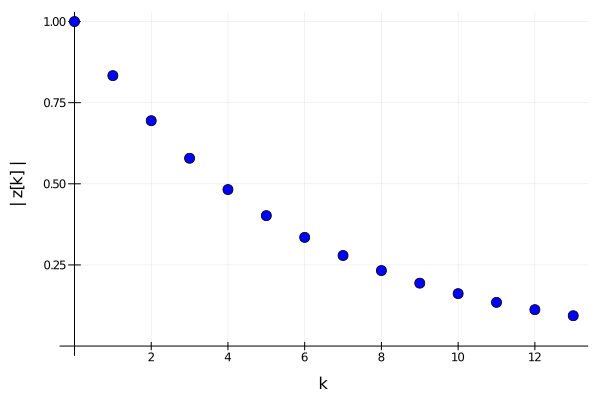
\includegraphics[width=\textwidth]{graphicsAppendices/CoolThings/SpiralIn02.png}
  \caption{$a = 1/2 + \im~2/3 = 0.83 e^{\im~ 0.93}$}
\end{subfigure}
\begin{subfigure}{.32\textwidth}
  \centering
  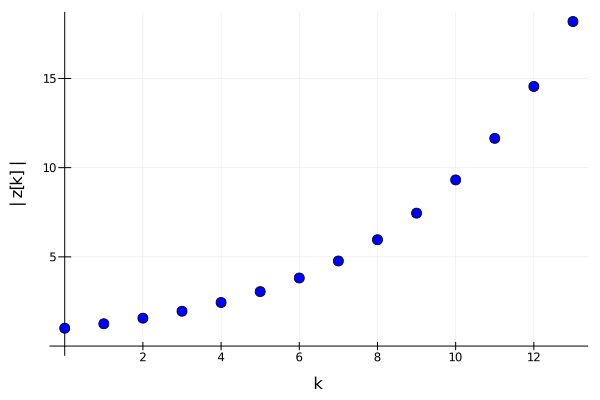
\includegraphics[width=\textwidth]{graphicsAppendices/CoolThings/SpiralOut02.png}
  \caption{$a = 3/4 + \im~ = 1.25 e^{\im~ 0.93}$}
\end{subfigure}
\begin{subfigure}{.32\textwidth}
  \centering
  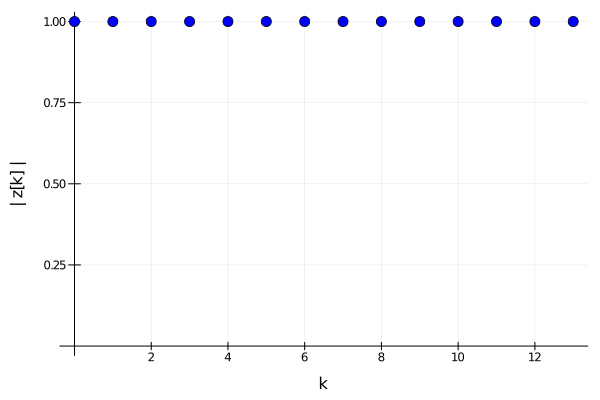
\includegraphics[width=\textwidth]{graphicsAppendices/CoolThings/Spiral02.png}
  \caption{$a = 3/5 + \im~4/5 = 1.0  e^{\im~ 0.93}$}
\end{subfigure}

\begin{subfigure}{.32\textwidth}
  \centering
  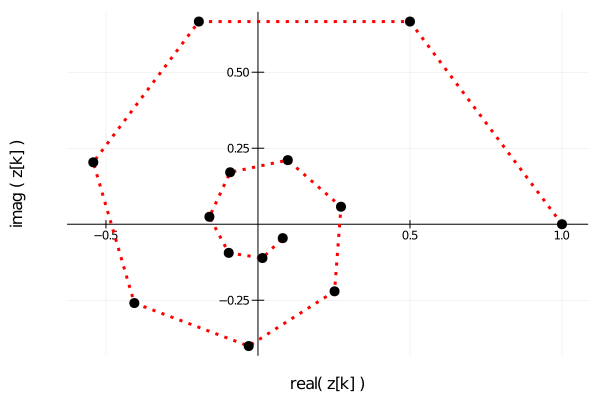
\includegraphics[width=\textwidth]{graphicsAppendices/CoolThings/SpiralIn01.png}
  \caption{$a = 3/5 + \im~4/5 = 1.0 \angle 53.1$ degrees}
\end{subfigure}
\begin{subfigure}{.32\textwidth}
  \centering
  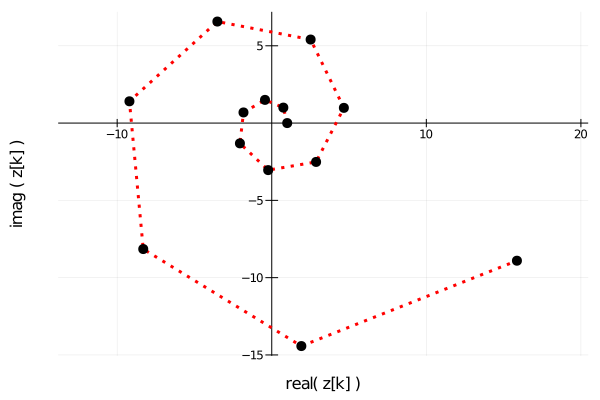
\includegraphics[width=\textwidth]{graphicsAppendices/CoolThings/SpiralOut01.png}
  \caption{$a = 3/4 + \im~ = 1.25 \angle 53.1$ degrees}
\end{subfigure}
\begin{subfigure}{.32\textwidth}
  \centering
  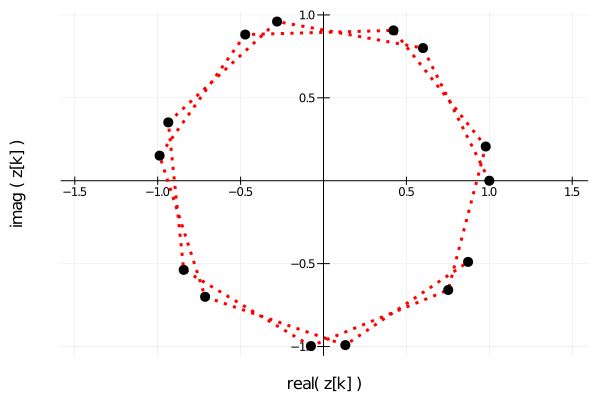
\includegraphics[width=\textwidth]{graphicsAppendices/CoolThings/Spiral01.png}
  \caption{$a = 3/5 + \im~4/5 = 1.0   \angle 53.1$ degrees}
\end{subfigure}

\caption{The solid dots illustrate the evolution of $z_k$ in \eqref{eq:IteratingComplexNumbers} and \eqref{eq:IteratingComplexNumbers02} when $a$ has magnitude less than one, greater than one, and equal to one, respectively. In each case, $z_0 = 1.0 + \im~0.0$ and the angle of $a$ was selected to be $53.1$ degrees; therefore the dots rotate counterclockwise. The red dashes are present to guide the eye in connecting the dots. In (f), the points lie on a circle of radius one.}
\label{fig:comparison_magnitude_of_a}
\end{figure}

\vspace*{0.2cm}

The following analysis supports the illustrations in Fig.~\ref{fig:comparison_magnitude_of_a}.

\vspace*{0.2cm}

\textbf{Case 1: |a|<1} We note that $\log(|a|^k) = k \log(|a|)$, and that $|a|<1 \implies \log(|a|) < 0.$ Hence, 
$$\lim_{k \to \infty} |a|^k = \lim_{k \to \infty} e^{k \log(|a|)} = 0. $$
\vspace*{0.2cm}


\textbf{Case 2: |a|>1} We note that $\log(|a|^k) = k \log(|a|)$, and that $|a|> 1 \implies \log(|a|) > 0.$ Hence, 
$$\lim_{k \to \infty} |a|^k = \lim_{k \to \infty} e^{k \log(|a|)} = \infty. $$ 
\vspace*{0.2cm}

\textbf{Case 3: |a|=1} We note that when $|a|=1$, then $|a|^k=1$ for all $k\ge 1$, and thus this case is clear. 
\vspace*{0.2cm}



\subsection{$\cp^n$, the Space of Complex Vectors}

$\cp^n$ sounds harder than it is. It's exactly $\real^n$ where  the scalars are complex numbers instead of real numbers. All the definitions of vector addition, linear combinations, spans, and linear independence are the same. We'll cover just a few of the basic ideas so that you get the idea.\\

Recall that we started by defining $\real^n$ as $n$-tuples of real numbers and then we identified it with column vectors of length $n$. We do that same here. 

\begin{equation}
\boxed{\cp^n:=\{(\alpha_1, \alpha_2, \ldots, \alpha_n)~|~\alpha_i \in \cp, 1\le i \le n \} \iff \left\{\begin{bmatrix} \alpha_1 \\ \alpha_2 \\ \vdots \\ \alpha_n\end{bmatrix} ~\Bigg|~  \alpha_i \in \cp, 1\le i \le n \right\}=:\cp^n}
\end{equation}

Consider two vectors $v_1\in \cp^n$ and $v_2\in \cp^n$. We define their \textbf{vector sum} by 
$$v_1+v_2=\begin{bmatrix} \alpha_1 \\ \alpha_2 \\ \vdots \\ \alpha_n\end{bmatrix}+  \begin{bmatrix} \beta_1 \\ \beta_2 \\ \vdots \\ \beta_n\end{bmatrix}:=\begin{bmatrix} \alpha_1 + \beta_1 \\ \alpha_2 + \beta_2 \\ \vdots \\ \alpha_n + \beta_n\end{bmatrix},$$
that is, we sum their respective components or entries. 
Let $\gamma$ be a complex number. Then we define 
$$\gamma v := \begin{bmatrix} \gamma \alpha_1 \\ \gamma \alpha_2 \\ \vdots \\\gamma \alpha_n\end{bmatrix}, $$
that is, to \textbf{multiply a complex vector by a complex number}, we multiply each of the components of the vector by the number, just as we do for real vectors.\\

Let $\{ v_1, v_2, \ldots, v_k\}$ be a collection of vectors in $\cp^n$. Then we define their \textbf{span} as 
$$\spanof{v_1, v_2, \ldots, v_k}:=\{ \alpha_1 v_1 + \alpha_2 v_2 + \cdots + \alpha_k v_k~|~ \alpha_i \in \cp, 1 \le i \le k\}. $$
The set of vectors  $\{ v_1, v_2, \ldots, v_k\}$ is \textbf{linearly independent} in the vector space $\cp^n$ if the only solution to 
$$\alpha_1 v_1 + \alpha_2 v_2 + \cdots + \alpha_k v_k=0 $$
is $\alpha_1=0 + \im~0, \alpha_2=0 + \im~0, \ldots, \alpha_k=0 + \im~0.$\\

The \textbf{norm} of a complex vector 
$$v=\begin{bmatrix} \alpha_1 \\ \alpha_2 \\ \vdots \\ \alpha_n\end{bmatrix}$$
is 
$$||v||:= \sqrt{\sum_{k=1}^{n} |\alpha_k|^2},$$
where, to be extra clear, $|\alpha_k|^2=\alpha_k \cdot \alpha_k^\ast.$ Moreover, if one defines the \textbf{complex conjugate of a vector} by taking the complex conjugate of each of its components, then 
$$||v||^2 = \left( v^\ast \right)^\top \cdot v, $$
and yes, the transpose simply takes the column vector to a row vector. 




\subsection{Iterating with Matrices: The Case for Eigenvalues and Eigenvectors}
\label{sec:CaseEigenvectors}

We now attempt to analyze the matrix versions of \eqref{eq:IteratingComplexNumbers} and \eqref{eq:IteratingComplexNumbers02}. Recall that you saw matrix difference equations in Project 3. Our real goal is to understand
\begin{equation}
    \label{eq:IteratingComplexMatrices}
x_{k+1}= A x_k,
\end{equation}
with $A$ an $n \times n$ real matrix and $x_0 \in \real^n$. But we'll see that allowing the entries of $A$ to be complex and $x_0 \in \cp^n$ does not change anything. \\

With this in mind, we rewrite \eqref{eq:IteratingComplexMatrices} first as 
$$x[k+1]= A x[k], $$
with the time index denoted in square brackets, Julia style! This will allow us to use a subscript for the components of $x$. Next, we replace $x[k]$ with $z[k]$ to emphasize that the we allow $z[k]$ to be a complex vector. We compute a few steps of $z[k+1]=A z[k]$ until the general pattern of its solution becomes clear:
\begin{equation}
    \label{eq:IteratingComplexMatricesB}
    \begin{aligned}
   z[1]&= A z[0]\\
   z[2]& = A z[1] = A^2 z[0] \\
   z[3]&= A z[2] = A^3 z[0]\\
   &~\vdots \\
   z[k]&=A^k z[0].
    \end{aligned}
\end{equation}
So far so good! Now, our challenges are:
\begin{itemize}
    \item give conditions on $A$ so that $||~z[k]~ ||$ contracts, blows up, or stays bounded as $k$ tends to infinity;
    \item even better, for a given initial condition $z[0]$, describe in detail the evolution of $z[k]$ for $k > 0$.
\end{itemize}

We'll start with a diagonal $n \times n $ matrix $A$, and for reasons that will become clear in the next section, we'll denote the entries on the diagonal by $\lambda$,
\begin{equation}
    \label{eq:diagonalAiteration}
    A= \left[\begin{array}{cccc} \lambda_1 & 0 & 0 & 0\\
0 & \lambda_2 & 0 & 0\\
0& 0& \ddots & 0\\
0& 0& 0 & \lambda_n\end{array}\right].
\end{equation}
We leave it as an exercise to compute that 
\begin{equation}
    \label{eq:diagonalAiteration02}
    A^2= \left[\begin{array}{cccc} \left(\lambda_1\right)^2 & 0 & 0 & 0\\
0 & \left(\lambda_2\right)^2 & 0 & 0\\
0& 0& \ddots & 0\\
0& 0& 0 & \left(\lambda_n\right)^2\end{array}\right],
\end{equation}
and once you have established \eqref{eq:diagonalAiteration02}, you will have no trouble believing that 
\begin{equation}
    \label{eq:diagonalAiteration03}
    A^k= \left[\begin{array}{cccc} \left(\lambda_1\right)^k & 0 & 0 & 0\\
0 & \left(\lambda_2\right)^k & 0 & 0\\
0& 0& \ddots & 0\\
0& 0& 0 & \left(\lambda_n\right)^k\end{array}\right].
\end{equation}\\

One thing we can do is observe that
\begin{equation}
    \label{eq:diagonalAiteration04}
    \begin{bmatrix} z_1[k] \\z_2[k] \\ \vdots \\ z_n[k]\end{bmatrix} =
  \left[\begin{array}{cccc} \left(\lambda_1\right)^k & 0 & 0 & 0\\
0 & \left(\lambda_2\right)^k & 0 & 0\\
0& 0& \ddots & 0\\
0& 0& 0 & \left(\lambda_n\right)^k\end{array}\right] \begin{bmatrix} z_1[0] \\z_2[0] \\ \vdots \\ z_n[0]\end{bmatrix}
\end{equation}
results in $n$ scalar equations of the form \eqref{eq:IteratingComplexNumbers}, namely,
\begin{equation}
    \label{eq:diagonalAiteration05}
    \boxed{
z_j[k]= (\lambda_j)^k z_j[0],~~1\le j \le n.}
\end{equation}

\vspace*{0.2cm} 
\begin{tcolorbox}
[title=\textbf{Linear Difference Equation with a Diagonal Matrix}]
The general solution to $z[k+1]= A z[k]$, $z[0]\in \cp^n$ is $z[k] = A^k z[0]$. When $A$ is diagonal, the solution is given in \eqref{eq:diagonalAiteration04} and \eqref{eq:diagonalAiteration05}. Based on these results and Chapter~\ref{sec:IteratingComplexnumbers}, we analyze three cases for $z_j[0] \neq 0$,
\begin{itemize}
    \item $|\lambda_j|<1 \implies |z_j[k]| \underset{k \to \infty}{\longrightarrow} 0$
    \item $|\lambda_j|>1 \implies |z_j[k]| \underset{k \to \infty}{\longrightarrow} \infty$
 \item $|\lambda_j|=1 \implies |z_j[k]|=|z_j[0]|, k \ge 0$.
\end{itemize}
\end{tcolorbox}

Being a ROB 101 student, having ``real'' matrices replaced by diagonal matrices must be a bit disconcerting! You'll be glad to know that it is really just a step to something kind of magical: most matrices can be factored as $A = M \Lambda M^{-1}$, where $\det(M)\neq 0$ and $\Lambda$ is diagonal, as in \eqref{eq:diagonalAiteration}. But we get ahead of ourselves!\\


\vspace*{0.2cm}

\begin{tcolorbox}[title = \textbf{Key features of a Diagonal Matrix: One way that Eigenvalues and Eigenvectors come about}]
Let $v_j = e_j$, where $e_j$ are the canonical basis vectors for either  $\real^n$ or $\cp^n$ (aka, columns of the $n \times n$ identity matrix). We have noted before that $A e_j = a_j^{\rm col}$. In our case, $ a_j^{\rm col} = \lambda_j e_j$. Hence, substituting in $v_j = e_j$, we arrive at the equation
\begin{equation}
    \label{eq:evaluesDiagonalMatrix}
    \boxed{
A v_j =\lambda_j v_j,~~1\le j \le n.}
\end{equation}
Equation \eqref{eq:evaluesDiagonalMatrix} is the defining relation for eigenvalues (denoted here by $\lambda_j$) and eigenvectors (denoted here by $v_j$). We further note that the set of vectors
$\{ v_1, v_2, \ldots, v_n\} $
is linearly independent and spans both $\real^n$ and $\cp^n$. Having a set of eigenvectors that forms a basis turns out to be a defining characteristic of matrices that are related to a diagonal matrix $\Lambda$ by a transformation of the form  $A = M \Lambda M^{-1}$.\\
\end{tcolorbox}

\vspace*{0.2cm}
\textbf{Remark:} If $ v \in \cp^n$ is an eigenvector, meaning $v \neq 0$ and there exists a $\lambda \in \cp$
such that \eqref{eq:evaluesDiagonalMatrix} holds, then we have that
\begin{align*}
    A v & = \lambda v\\
    A^2 v & = A (\lambda v) = \lambda  A  v  = (\lambda)^2 v\\
    & ~~\vdots \\
    A^k v & = (\lambda)^k v
\end{align*}
and hence we can analyze convergence for the difference equation $z[k+1]=A z[k]$, $z[0]=v$, even when $A$ is not diagonal.
\vspace*{0.2cm}

\textbf{Remark:} Suppose that $A$ is real and that $\lambda \in \cp$ and $ v \in \cp^n$, satisfy $Av = \lambda v$ and $v\neq 0$. Even though the eigenvalue and eigenvector are complex, their real and imaginary parts are very relevant to computations in $\real^n$. Decompose $\lambda$ and $v$ into their real and imaginary parts, viz
\begin{equation}
    \label{eq:JordanSubspaceStuff}
    \begin{aligned}
    \lambda&=: \lambda_{\rm Re} + \im ~\lambda_{\rm Im}\\
    v&=: v_{\rm Re} + \im ~v_{\rm Im}.
    \end{aligned}
\end{equation}
Then
\begin{equation}
    \label{eq:JordanSubspaceStuff02}
    \begin{aligned}
   A v_{\rm Re} &= \repart{A v} =\lambda_{\rm Re} \cdot v_{\rm Re} - \lambda_{\rm Im} \cdot v_{\rm Im}\\
    A v_{\rm Im} &= \impart{A v} =  \lambda_{\rm Im} \cdot v_{\rm Re} + \lambda_{\rm Re} \cdot v_{\rm Im}.
    \end{aligned}
\end{equation}
Hence, 
\begin{equation}
    \label{eq:JordanSubspaceStuff03}
     \begin{bmatrix}
      A v_{\rm Re}\\ A v_{\rm Im}
    \end{bmatrix} = \left[ \begin{array}{rr} \lambda_{\rm Re} I_n & - \lambda_{\rm Im} I_n\\
     \lambda_{\rm Im}I_n &  \lambda_{\rm Re} I_n\end{array} \right] \begin{bmatrix}
      v_{\rm Re}\\ v_{\rm Im}
    \end{bmatrix}. 
\end{equation}
If we write $\lambda = |\lambda| e^{\im~\theta} = |\lambda| \cos(\theta) + \im ~|\lambda| \sin(\theta) $, then \eqref{eq:JordanSubspaceStuff03} can be rewritten as
\begin{equation}
    \label{eq:JordanSubspaceStuff04}
    \begin{bmatrix}
     A v_{\rm Re}\\ A v_{\rm Im}
    \end{bmatrix} =  |\lambda| \underbrace{\left[ \begin{array}{rr}\cos(\theta) I_n & - \sin(\theta) I_n\\
    \sin(\theta)I_n &  \cos(\theta) I_n\end{array} \right]}_{R(\theta)} \begin{bmatrix}
      v_{\rm Re}\\ v_{\rm Im}
    \end{bmatrix},
\end{equation}
where $R(\theta)^\top \cdot R(\theta)=R(\theta) \cdot R(\theta)^\top = I_{2n}$, and hence $R(\theta)$ is an orthogonal matrix. This shows how the complex aspect of the eigenvalue and eigenvector manifests itself as a ``kind of rotation'' of vectors in the two dimensional subspace 
$$\spanof{v_{\rm Re}, v_{\rm Im}} $$
by $R(\theta)$, in addition to the scaling by $|\lambda|$. A second benefit of the latter expression is that we then have 
\begin{equation}
    \label{eq:JordanSubspaceStuff05}
     \begin{bmatrix}
     A^k v_{\rm Re}\\ A^k v_{\rm Im}
    \end{bmatrix} =  |\lambda|^k \underbrace{ \left[ \begin{array}{rr}\cos(k \theta) I_n & - \sin (k\theta) I_n\\
    \sin(k \theta)I_n &  \cos(k \theta) I_n\end{array} \right]}_{R(k\theta)} \begin{bmatrix}
      v_{\rm Re}\\ v_{\rm Im}
    \end{bmatrix}.
\end{equation}
Figure~\ref{fig:SpanRealImaginaryParts} illustrates a case where $\lambda=0.9803 \pm \im~ 0.0965= 0.985 \angle 5.6$ degrees. The rotating and decaying nature of the solution is clearly seen in the figure. The reader should compare Figs.~\ref{fig:comparison_magnitude_of_a}-(a) and -(d) with Fig.~\ref{fig:SpanRealImaginaryParts}. 

\vspace*{0.2cm}



\begin{figure}[htb!]
\centering
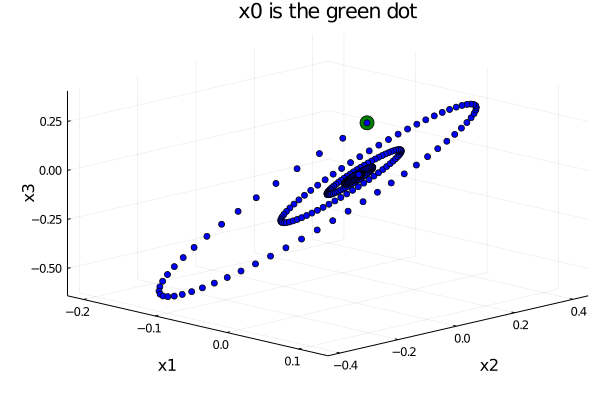
\includegraphics[width=0.8\textwidth]{graphicsAppendices/CoolThings/DecayingWhileOscillating01.png}
\caption[]{The eigenvalues of a real $3 \times 3$ matrix are computed to be $0.9803 \pm \im~ 0.0965$ and $ 1.100$. The initial condition in green was chosen to be a linear combination of the real and imaginary parts of an eigenvector corresponding to the complex pair of eigenvalues. The resulting solution of \eqref{eq:IteratingComplexMatricesB} evolves in the plane defined by $\spanof{v_{\rm Re}, v_{\rm Im}}$ as indicated by  \eqref{eq:JordanSubspaceStuff03} through \eqref{eq:JordanSubspaceStuff05}. This is very analogous to how complex numbers, when iterated, evolve in the Complex Plane.}
\label{fig:SpanRealImaginaryParts}
\end{figure}


\section{Eigenvalues and Eigenvectors}
\label{sec:EigenStuff}

The study of eigenvalues and eigenvectors is very traditional in Linear Algebra courses. We skipped very important aspects of them in the main portion of the book for a few reasons: (1) time is limited; (2) they get complicated really fast; and (3) their most important applications are the evolution of linear difference equations and the Singular Value Decomposition (SVD), neither of which were covered in the main portion of the text. The usual illustrative application of eigenvalues and eigenvectors is to ``diagonalize'' a matrix, which we treated indirectly in Chapter~\ref{eq:xExpandedEigenBasisA}. In the context of Chapter~\ref{sec:CaseEigenvectors} and your Segway Project, it does make sense. \\

Just in case you are starting here and skipped Appendix~\ref{sec:ComplexNumbers} entirely, we start from the beginning.

\subsection{General Square Matrices}

\textbf{Temporary Def.}~ Let $A$ be an $n\times n$ matrix with real coefficients. A scalar $\lambda \in \real$ is an \textbf{eigenvalue} (e-value) of $A$, if there exists a non-zero vector $v \in \real^{n}$ such that $A \cdot v=\lambda v$. Any such vector $v$ is called an \textbf{eigenvector} (e-vector) associated with $\lambda$.\\

We note that if $v$ is an e-vector, then so is $\alpha v$ for any $\alpha \neq 0$, and therefore, e-vectors are not unique. To find eigenvalues, we need to have conditions under which there exists $v \in \real^n$, $v \neq 0$, such that $A \cdot v=\lambda v$. Here they are,
    \begin{equation*}
        A \cdot v=\lambda v \iff(\lambda I-A)\cdot v=0 \overset{v\neq 0}{\iff} \det(\lambda I-A)=0.
    \end{equation*}
    
    
\begin{example}
\label{ex:Eigen01} Let $A$ be the $2 \times 2$ real matrix
 $A=\left[\begin{array}{rr}
    0 & 1\\
    -1 & 0
    \end{array}\right].$
Determine, if any, its e-values and e-vectors. 
\end{example}

\textbf{Solution:} To find e-values, we need to solve 
$$\det(\lambda I-A)= \left| \begin{array}{rr}
    \lambda & -1\\
    1 &\lambda
    \end{array} \right| =\lambda^2+1=0.$$
    We compute the discriminant of this quadratic equation and we find
    $$b^2-4ac = -4 <0,$$
    and therefore there are no real solutions. Hence, by our \textit{temporary definition}, this $2 \times 2$ real matrix does not have any e-values, and hence, neither does it have any e-vectors.\\
    
    If we were to allow e-values to be complex numbers, then we'd have two e-values corresponding to the two complex solutions of the quadratic equation $\lambda^2+1=0$, namely, $\lambda_1 = \im$ and $\lambda_2 = -\im$.\\
    
    We'll see shortly that we'll also need to allow the e-vectors to have complex entries. Hence, we need to generalize our temporary definition. 
\Qed
    
    
\begin{tcolorbox}[title=\textbf{Permanent Definition of Eigenvalues and Eigenvectors}]
 Let $A$ be an $n\times n$ matrix with real or complex coefficients. A scalar $\lambda \in  \cp$ is an \textbf{eigenvalue} (e-value) of $A$, if there exists a non-zero vector $v \in \cp^{n}$ such that $Av=\lambda v$. Any such vector $v$ is called an \textbf{eigenvector} (e-vector) associated with $\lambda$. \\
 
 Eigenvectors are not unique.\\
 
 \begin{itemize}
\item To find e-values, we solve $\det(\lambda I - A)=0$ because
    \begin{equation}
        A \cdot v=\lambda v \iff(\lambda I-A)\cdot v=0 \overset{v\neq 0}{\iff} \det(\lambda I-A)=0.
    \end{equation}
\item To find e-vectors, we find any non-zero $v\in \cp^n$ such that 
\begin{equation}
\label{eq:EvectorDef}
    (\lambda I-A)\cdot v=0.
\end{equation}
\end{itemize}
Of course, if you prefer, you can solve $(A - \lambda I)v=0$ when seeking e-vectors.
\end{tcolorbox}

\vspace*{0.5cm}
\begin{tcolorbox}[sharp corners, colback=green!30, colframe=green!80!blue, title=\textbf{\large Fundamental Theorem of Algebra (and a bit More)}]
Let $A$ be an $n\times n$ matrix with real or complex coefficients. Then the following statements are true
\begin{itemize}
    \item $\det(\lambda I - A) = \lambda^n + \alpha_{n-1} \lambda^{n-1} + \cdots \alpha_1 \lambda + \alpha_0$, and if $A$ is real, so are the coefficients $\alpha_{n-1}, \ldots, \alpha_0.$
    
    \item The degree $n$ polynomial $\lambda^n + \alpha_{n-1} \lambda^{n-1} + \cdots \alpha_1 \lambda + \alpha_0$ has $n$ roots $\lambda_1, \ldots, \lambda_n \in \cp$ such that
    $$\det(\lambda I - A) = (\lambda - \lambda_1) (\lambda - \lambda_2) \cdots (\lambda - \lambda_n). $$
    Each of the roots $\lambda_i$, $1 \le i \le n$, is an e-value of $A$.
    
    \item The e-values $\{\lambda_1, \ldots, \lambda_n\}$ are said to be \textbf{distinct} if $\lambda_i \neq \lambda_k$ for all $i \neq k$.
    
    \item If $\lambda_i=\lambda_k$ for some $i \neq k$, then $\lambda_i$ is a \textbf{repeated e-value}. The e-values can then be grouped into $1\le p \le n $ sets of distinct roots $ \{\lambda_1, \ldots, \lambda_p \} $ such that 
    $$\det(\lambda I - A) = (\lambda - \lambda_1)^{m_1} (\lambda - \lambda_2)^{m_2} \cdots (\lambda - \lambda_p)^{m_p}. $$
    The integer $m_i$ is called the \textbf{algebraic multiplicity} of $\lambda_i$ and their sum satisfies
    $m_1 + m_2 + \cdots + m_p = n.$
    
    \item An e-vector associated with $\lambda_i$ is computed by finding non-zero solutions to \eqref{eq:EvectorDef}. 
    
     \item If the matrix $A$ is real, then the e-values occur in \textbf{complex conjugate pairs}, that is, if $\lambda_i$ is an e-value then so is $\lambda^\ast_i$.
    
    \item If the matrix $A$ is real and the e-value $\lambda_i$ is real, then the e-vector $v_i$ can always be chosen to be real, that is, $v_i \in \real^n$ instead of $v_i \in \cp^n$. 
    
    \item There will always be at least one non-zero solution to \eqref{eq:EvectorDef}, and because any non-zero multiple of a solution is also a solution, there will always be an infinite number of solutions to \eqref{eq:EvectorDef}. 
    
    \item If $\lambda_i$ is a repeated e-value with algebraic multiplicity $m_i$, then the number of linearly independent e-vectors associated with $\lambda_i$ is upper bounded by $m_i$. Another way to say this is, $1 \le \dim\left({\rm Null}(A-\lambda_i I) \right) \le m_i$.
    
    \item \textbf{In Julia}, after $\texttt{using LinearAlgebra}$, the commands are $\Lambda = \texttt{eigvals(A)}$ and $V=\texttt{eigvecs(A)}$
\end{itemize}

\end{tcolorbox}

\begin{example}
\label{ex:Eigen02} Let $A$ be the $2 \times 2$ real matrix that we treated in Example~\ref{ex:Eigen01}, namely,
 $A=\left[\begin{array}{rr}
    0 & 1\\
    -1 & 0
    \end{array}\right].$
Determine its e-values and e-vectors in the sense of our ``permanent'' definition. 
\end{example}

\textbf{Solution:} As in Example~\ref{ex:Eigen01}, to find e-values, we solve 
$$\det(\lambda I-A)= \left| \begin{array}{rr}
    \lambda & -1\\
    1 &\lambda
    \end{array} \right| =\lambda^2+1=0.$$
   We apply the quadratic equation and determine $\lambda_1 = \im$ and $\lambda_2= - \im$.  To find the eigenvectors, we solve 
   $$(A-\lambda_{i}I)v_i=0.$$
    The eigenvectors are $$v_{1}=\left[\begin{array}{c}
        1\\
        \im
    \end{array}\right],v_{2}=\left[\begin{array}{c}
        1\\
        -\im
    \end{array}\right].$$
Note that the eigenvalues and eigenvectors each form complex conjugate pairs. Indeed,
$$\lambda_2 = \lambda_1^\ast~~\text{and}~~v_2 = v_1^\ast. $$
\Qed

\begin{example}
\label{ex:Eigen03} Let $A$ be the $n \times n$ identity matrix. Determine its e-values and e-vectors.
\end{example}

\textbf{Solution:} $\det(\lambda I - I)=\det((\lambda-1)I_=0 \iff \lambda = 1.$ Alternatively, you can compute that $\det(\lambda I - I) = (\lambda -1)^n.$ Hence, the e-value $\lambda=1$ is repeated $n$ times, that is, $m_1=n$. What are the e-vectors? We seek to solve 
$$(A-\lambda I)\cdot v = 0 \iff (I - 1\cdot I) \cdot v = 0 \iff 0_n \cdot v=0, $$
where $0_n$ is the $n \times n$ matrix of all zeros! Hence, any non-zero vector $v\in \real^n$ is an e-vector. Moreover, if $\{v_1, \ldots, v_n \}$ is a basis for $\real^n$, then $\{v_1, \ldots, v_n \}$ is a set of $n$ linearly independent e-vectors associated with $\lambda_1=1$.
\Qed

\begin{example}
\label{ex:Eigen04} Let $a\in \real$ be a constant and let $A$ be the $4 \times 4$ matrix below. Determine its e-values and e-vectors.
$$A= \left[\begin{array}{cccc} a & 1 & 0 & 0\\
0 & a & 1 & 0\\
0& 0& a & 1\\
0& 0& 0 & a\end{array}\right]. $$
\end{example}

\textbf{Solution:} To find the e-values, we solve
$$\det(\lambda I - A) =  \det\left(\left[\begin{array}{cccc} (\lambda-a) & -1 & 0 & 0\\
0 & (\lambda-a) & -1 & 0\\
0& 0& (\lambda-a) & -1\\
0& 0& 0 & (\lambda-a)\end{array}\right] \right) = (\lambda-a)^4=0,$$
and hence there is one distinct e-value $\lambda_1 = a$. To solve for e-vector(s) we consider
$$0=(A - a I) \cdot v = \left[\begin{array}{cccc} 0 & 1 & 0 & 0\\
0 & 0 & 1 & 0\\
0& 0& 0 & 1\\
0& 0& 0 & 0\end{array}\right] \cdot v$$
and we find that the only solutions are multiples of 
$$v=\left[\begin{array}{c} 1 \\ 0 \\ 0 \\ 0 \end{array}\right].$$
\Qed
\vspace*{0.5cm}
\begin{tcolorbox}
We've seen the extremes! A matrix with a single distinct e-value and a complete set of e-vectors (there were $n$ linearly independent e-vectors associated with the e-value), and another matrix with a single distinct e-value, but only one linearly independent e-vector associated with it. 
\end{tcolorbox}
\vspace*{0.5cm}
\begin{tcolorbox}[sharp corners, colback=green!30, colframe=green!80!blue, title=\textbf{\large When the e-values are Distinct, the e-vectors form a Basis}]
Let $A$ be an $n \times n$ matrix with coefficients in $\real$ or $\cp$. If the e-values $\{ \lambda_1,\ldots, \lambda_n \}$ are distinct, that is, $\lambda_i \neq \lambda_j $ for all $1 \le i \neq j \le n$, then the e-vectors $\{ v_1,\ldots,v_n \}$ are linearly independent in ($\cp^n$,$\cp$).\\

\textbf{Restatement of the result:} If $\{ \lambda_1,\ldots,\lambda_n \}$ are distinct, then $\{ v_1,\ldots,v_n \}$ is a basis for ($\cp^n$,$\cp$). If $A$ is real and its e-values are real, then the e-vectors can be chosen to be real and they form a basis for $\real^n$.
\end{tcolorbox}

\subsection{Real Symmetric Matrices}
\label{sec:RealSymmetricMatrices}

We recall that a real  $n\times n$ matrix $A$ is \textbf{symmetric} if $A^\top=A$. E-values and e-vectors of symmetric matrices have nicer properties than those of general matrices. 

\begin{tcolorbox}[title=\textbf{\large E-values and E-vectors of Symmetric Matrices}]

\begin{itemize}
    \item The e-values of a symmetric matrix are real. Because the e-values are real and the matrix is real, we can always chose the e-vectors to be real. Moreover, we can always normalize the e-vectors to have \textbf{norm one}.
    
    \item Just as with general matrices, the e-values of a symmetric matrix may be distinct or repeated. However, even when an e-value $\lambda_i$ is repeated $m_i$ times, there are always $m_i$ linearly independent e-vectors associated with it. By applying Gram-Schmidt, we can always chose these e-vectors to be \textbf{orthonormal}.
    
    \item E-vectors associated with distinct e-values are automatically orthogonal. To be clear, $$ \big(A^\top = A,~Av_i = \lambda_i v_i, Av_k = \lambda_k v_k,~\text{and} ~~\lambda_i \neq \lambda_k \big) \implies v_i \perp v_k.$$
    Since we can assume they have length one, we have that the e-vectors are \textbf{orthonormal}.
    
    \item \textbf{In summary}, when $A$ is symmetric, there is always an orthonormal basis $\{v_1, v_2, \ldots, v_n \}$ for $\real^n$ consisting of e-vectors of $A$. In other words, for all $1 \le i \le n$, $Av_i = \lambda_i v_i$, $||v_i||=1$, and for $k \neq i$, $v_k \perp v_i$.
\end{itemize}

\end{tcolorbox}

\vspace*{.2cm}

\begin{tcolorbox}[sharp corners, colback=green!30, colframe=green!80!blue, title=\textbf{\large Factoring a Symmetric Matrix}]

For every real $n \times n$ symmetric matrix $A$, there exists an $n \times n $ diagonal matrix $\Lambda$ and an $n \times n $ orthogonal matrix $Q$ such that
\begin{equation}
    \label{eq:FactorSymmetricA}
    A = Q \cdot \Lambda \cdot Q^\top.
\end{equation}
Moreover, 
$$\Lambda=\left[\begin{array}{cccc}
    \lambda_1 & 0  & \cdots & 0\\
    0 & \lambda_2 &  \cdots & 0 \\
    \vdots & \vdots & \ddots & 0\\
    0 &  0 & \cdots  & \lambda_n
    \end{array}\right] ~~\text{and}~~Q = \left[\begin{array}{ccccc}
  v_1 & v_2  & \ldots & v_n
    \end{array}\right]$$
% $$\Lambda=\left[\begin{array}{ccccc}
%     \lambda_1 & 0 & 0 & \cdots & 0\\
%     0 & \lambda_2 & 0 & \cdots & 0 \\
%     0 & 0 & \lambda_3  & \cdots & 0 \\
%     \vdots & \vdots & \vdots & \ddots & 0\\
%     0 & 0 & 0 & \cdots  & \lambda_n
%     \end{array}\right] ~~\text{and}~~Q = \left[\begin{array}{ccccc}
%   v_1 & v_2 & v_3 & \ldots & v_n
%     \end{array}\right]$$
are constructed from the e-values of $A$ and a corresponding set of orthonormal e-vectors.\\


\textbf{Remark 01:} From \eqref{eq:FactorSymmetricA}, $\det(A) = \det(Q) \cdot \det(\Lambda) \cdot \det(Q^\top) = \det(\Lambda) = \lambda_1 \cdot \lambda_2 \cdots \lambda_n$. Hence, a symmetric real matrix $A$ is invertible if, and only if, all of its e-values are non-zero. Moreover, in this case
$$A^{-1}=Q \cdot \Lambda^{-1} \cdot Q^\top. $$
While a similar result holds for general square matrices, it requires inverting the matrix formed by stacking the e-vectors as columns, and hence is not numerically attractive. For symmetric matrices, the corresponding inverse is computed via a matrix transpose.\\


\textbf{Remark 02:} Using the fact that matrix multiplication can be realized by summing over the product of columns times rows, \eqref{eq:FactorSymmetricA} can be rewritten as 
\begin{equation}
    \label{eq:FactorSymmetricA02}
    A = \sum_{i=1}^n \lambda_i \left( v_i \cdot v_i^\top\right).
\end{equation}
Equations~\eqref{eq:FactorSymmetricA} and ~\eqref{eq:FactorSymmetricA02} parallel results we will develop for the Singular Value Decomposition or (SVD). Equation~\eqref{eq:FactorSymmetricA} factors $A$ into a product of three terms consisting of two orthogonal matrices and a diagonal matrix, while \eqref{eq:FactorSymmetricA02} is an expansion of $A$ into ``rank one'' matrices. 

\end{tcolorbox}



\section{Positive Definite Matrices}
\label{sec:PosDefMatrices}

\begin{tcolorbox}[title= \textbf{Some Definitions and Facts}]

\begin{enumerate}
    \item[{\bf Def.}]  Let $P$ be an $n \times n$ real matrix and $x \in \real^n.$ Then $x^\top Px$ is called a \textbf{quadratic form}.
    
    \item[{\bf Def.}] An $n \times n$ matrix $S$ is \textbf{skew symmetric} if $S^\top=-S$.
    
    \item[{\bf Fact}]  If $S$ is skew symmetric, then $x^\top S x=0$ for all $x \in \real^n$.
    
    \item[{\bf Fact}] Let $P$ an $n \times n$ real matrix and write
    $$P = \frac{1}{2} \left(P + P^\top   \right) + \frac{1}{2} \left(P - P^\top   \right).$$
    Then $\left(P + P^\top   \right)$ is symmetric, $ \left(P - P^\top   \right)$ is skew symmetric, and we see that every (real) square matrix can be written as the sum of a symmetric matrix and a skew symmetric matrix. 
  
      \item[{\bf Fact}] Let $P$ an $n \times n$ real matrix. Then, for all $x\in \real^n$
      $$x^\top Px=  \frac{1}{2}  x^\top \left(P + P^\top   \right)x.$$
      Hence, a quadratic form only depends on the symmetric part of a matrix. \\
      
      \textbf{Consequence:} When working with a quadratic form, $x^\top P x$, one \textbf{ALWAYS} assumes that the matrix $P$ is symmetric. Allowing the matrix to be non-symmetric does not increase the generality of the notion of a quadratic form. This is because $x^\top Px=  \frac{1}{2}  x^\top \left(P + P^\top   \right)x$ implies that one can always replace $P$ with its symmetric part!
      
      \item[{\bf Fact}] For an $n \times n$ symmetric real matrix $P$ with e-values $\lambda_1, \ldots, \lambda_n$, let $\lambda_{\rm max}:= \max_{1 \le i \le n} \lambda_i$ and $\lambda_{\rm min}:= \min_{1 \le i \le n} \lambda_i$ be the max and min, respectively over the e-values. Then, for all $x\in \real^n$,
      \begin{equation}
          \label{eq:SymmetricBoundsEvalues}
          \lambda_{\rm min}~ x^\top x \le x^\top P x \le \lambda_{\rm max}~ x^\top x.
      \end{equation}
      Because $x^\top x = ||x||^2$, the above expression is also commonly written as
      $$  \lambda_{\rm min}~ ||x||^2 \le x^\top P x \le \lambda_{\rm max}~ ||x||^2.$$
      Both are useful.
\end{enumerate}
\end{tcolorbox}

\vspace*{.2cm}

Equation~\eqref{eq:SymmetricBoundsEvalues} is established by choosing an orthonormal set of e-vectors for $P$, $\{v_1, \ldots, v_n \}$, which we know forms a basis for $\real^n$. Hence, for all $x\in \real^n,$ there exist coefficients $\alpha_1, \dots, \alpha_n$ such that $x = \alpha_1 v_1 + \cdots + \alpha_n v_n$. Then, using the two facts we have at our disposal, namely (a) $\{v_1, \ldots, v_n \}$ is orthonormal and (b), $Av_i = \lambda_i v_i$, we compute
\begin{align*}
    x^\top x =& \alpha_1^2 + \cdots + \alpha_n^2\\
      x^\top Px =& \lambda_1 \alpha_1^2 + \cdots + \lambda_n \alpha_n^2.
\end{align*}
It follows that 
$$\lambda_{\rm min} x^\top x =  \lambda_{\rm min} \alpha_1^2 + \cdots + \lambda_{\rm min} \alpha_n^2 \le  \lambda_1 \alpha_1^2 + \cdots + \lambda_n \alpha_n^2 \le \lambda_{\rm max} \alpha_1^2 + \cdots + \lambda_{\rm max}\alpha_n^2 = \lambda_{\rm max} x^\top x, $$
showing that \eqref{eq:SymmetricBoundsEvalues} holds.

\vspace*{.2cm}


\begin{tcolorbox}[sharp corners, colback=green!30, colframe=green!80!blue, title={ \bf \large Positive Definite and Semidefinite Matrices} ]

\begin{enumerate}
    \item[{\bf Def.}]  A real symmetric matrix $P$ is \textbf{positive definite}, if for all $x \in \real^n$, $x\neq 0 \implies x^\top Px>0.$ The common notation for such matrices is $P > 0.$
    
    \item[{\bf Def.}]  A real symmetric matrix $P$ is positive semidefinite, if for all $x \in \real^n \implies x^\top Px\ge0.$  The common notation for such matrices is $P \ge 0.$\\
    
 \textbf{ From~\eqref{eq:SymmetricBoundsEvalues}, we arrive at the following facts.}


 \item[{\bf Fact}]   A symmetric matrix $P$ is positive definite if, and only if, all of its eigenvalues are greater than $0$.
 
 
 \item[{\bf Fact}]   A symmetric matrix $P$ is positive semidefinite if, and only if, all of its eigenvalues are greater than or equal to $0$.
 \end{enumerate}
\end{tcolorbox}

\begin{example}
\label{ex:P0sDef01} Determine, which, if any, of the following matrices are positive definite or positive semidefinite.
$$ P_1 = \left[ \begin{array}{rr} 2 & -1 \\	-1 & 2 \end{array} \right],  P_2 = \left[ \begin{array}{rr} 1 & 2 \\	2 & 1 \end{array} \right], P_3 = \left[ \begin{array}{rr} 4 & 2 \\	2 & 1 \end{array} \right],  P_4 = \left[ \begin{array}{rr} 4 & 1 \\	3 & 4 \end{array} \right] $$
\end{example}

\textbf{Solution:} Because $P_4$ is not symmetric, it cannot be positive definite or positive semidefinite! Using Julia, we compute the e-values of $P_1$, $P_2$, and $P_3$
\begin{align*}
    P_1 &\implies \lambda_1 = 1, \lambda_2 = 3 \implies P > 0\\
    P_2 &\implies \lambda_1 = -1, \lambda_2 =3 \implies P \not \ge 0~\text{(neither positive semidefinite nor positive definite)} \\
    P_3 &\implies \lambda_1 = 0, \lambda_2 = 5\implies P \ge 0.
\end{align*}
We note that $P$ being positive definite does NOT mean that all of its entries have to be positive! $P$ can have entries with negative values and still be positive definite. We note that all of the entries of $P$ being positive does NOT imply that $P$ is even positive semidefinite.  
\Qed. 


\vspace*{.2cm}

Computing e-values is a terrible way to determine if a matrix is positive definite or not. The following facts imply that LDLT Factorization can be applied to positive definite and positive semidefinite matrices.

\begin{tcolorbox}[title=\textbf{\large \textcolor{red}{More on} Positive Definite and Semidefinite Matrices}]

\begin{enumerate}
    \item[{\bf Fact}]   A symmetric $n \times n$  matrix  $P$ is positive semidefinite if, and only if, there exists a $k \times n$ matrix $N$ such that $N^\top \cdot N = P.$\\
 
  
  \item[{\bf Fact}]   A symmetric $n \times n$ matrix $P$ is positive definite if, and only if, there exists an $n \times n$ matrix $N$ with linearly independent columns such that $N^\top \cdot N = P.$\end{enumerate}
\end{tcolorbox}

\vspace*{.2cm}
Turning these ideas into algorithmic form gives the following:

\begin{tcolorbox}[sharp corners, colback=green!30, colframe=green!80!blue,  title= \textbf{\large LDLT or LU Factorization to Check ${\bf P > 0}$}]
 Here are two better ways to test whether a matrix is positive definite, positive semidefinite, or neither:
\begin{itemize}
    \item From Chapter~\ref{sec:NumberLinIndepVectors}, we can do the LDLT factorization of $P$, namely
    $$Q\cdot P \cdot Q^\top = L \cdot D \cdot L^\top, $$
    where we have used $Q$ to denote the row permutation matrix because $P$ is being used for a symmetric matrix. Then $P >0 \iff D>0$, where $D$ is diagonal. 
    \item Straight up LU with no permutations at all:  The key fact is that, if an $n \times n$ matrix $P$ is symmetric and invertible, then it can be written as
$$ P = L \cdot U;$$
\textbf{you can do the factorization without permuting any of the rows of $\mathbf{P}$}. Moreover, there is always a diagonal matrix $D$ such that
$$ U = D \cdot L^\top.$$
Determining $D$ from $U$ is trivial: you just normalize by the diagonal of $U$. Then, $P=L \cdot D \cdot L^\top$ and
$$P > 0 \iff L \cdot D \cdot L^\top>0 \iff D > 0,~\text{that is, all of the entries on the diagonal of }D~\text{are positive}. $$
\item If the LU Factorization without permutations fails, then $P$ is not positive definite, but could be positive semidefinite. To rule out the latter, you need to run the full LDLT algorithm and check that the diagonal of $D$ has at least one negative entry or not.
\end{itemize}
\end{tcolorbox}
\vspace*{.2cm}

\begin{example}
\label{ex:P0sDef02} Using the LU Factorization without row permutations, determine if the randomly generated symmetric matrix $P$ is positive definite or not.
$$ P=
\left[
\begin{array}{ccccc}
8.241e-01 & 1.171e+00 & 1.117e+00 & 1.706e+00 & 1.021e+00 \\
1.171e+00 & 1.574e+00 & 8.547e-01 & 1.102e+00 & 2.871e-01 \\
1.117e+00 & 8.547e-01 & 1.238e+00 & 7.506e-01 & 1.291e+00 \\
1.706e+00 & 1.102e+00 & 7.506e-01 & 2.943e-01 & 9.570e-01 \\
1.021e+00 & 2.871e-01 & 1.291e+00 & 9.570e-01 & 1.448e+00 \\
\end{array}
\right].$$

\end{example}

\textbf{Solution:} We do the LU Factorization without permutations and obtain
\begin{align*}
    L&=\left[
\begin{array}{ccccc}
1.000e+00 & 0.000e+00 & 0.000e+00 & 0.000e+00 & 0.000e+00 \\
1.421e+00 & 1.000e+00 & 0.000e+00 & 0.000e+00 & 0.000e+00 \\
1.356e+00 & 8.151e+00 & 1.000e+00 & 0.000e+00 & 0.000e+00 \\
2.070e+00 & 1.469e+01 & 1.616e+00 & 1.000e+00 & 0.000e+00 \\
1.239e+00 & 1.294e+01 & 1.649e+00 & 5.893e-01 & 1.000e+00 \\
\end{array}
\right] \bigskip \\
U&=\left[
\begin{array}{rrrrr}
8.241e-01 & 1.171e+00 & 1.117e+00 & 1.706e+00 & 1.021e+00 \\
0.000e+00 & -8.990e-02 & -7.328e-01 & -1.321e+00 & -1.164e+00 \\
0.000e+00 & 0.000e+00 & 5.696e+00 & 9.203e+00 & 9.393e+00 \\
0.000e+00 & 0.000e+00 & 0.000e+00 & 1.296e+00 & 7.636e-01 \\
0.000e+00 & 0.000e+00 & 0.000e+00 & 0.000e+00 & -6.909e-01 \\
\end{array}
\right]
\end{align*}

We extract the diagonal of $U$ and we form $D \cdot L^\top$
\begin{align*}
    D &= \left[
\begin{array}{rrrrr}
8.241e-01 & 0.000e+00 & 0.000e+00 & 0.000e+00 & 0.000e+00 \\
0.000e+00 & -8.990e-02 & 0.000e+00 & 0.000e+00 & 0.000e+00 \\
0.000e+00 & 0.000e+00 & 5.696e+00 & 0.000e+00 & 0.000e+00 \\
0.000e+00 & 0.000e+00 & 0.000e+00 & 1.296e+00 & 0.000e+00 \\
0.000e+00 & 0.000e+00 & 0.000e+00 & 0.000e+00 & -6.909e-01 \\
\end{array}
\right] \bigskip \\
D \cdot L^\top & = \left[
\begin{array}{rrrrr}
8.241e-01 & 1.171e+00 & 1.117e+00 & 1.706e+00 & 1.021e+00 \\
0.000e+00 & -8.990e-02 & -7.328e-01 & -1.321e+00 & -1.164e+00 \\
0.000e+00 & 0.000e+00 & 5.696e+00 & 9.203e+00 & 9.393e+00 \\
0.000e+00 & 0.000e+00 & 0.000e+00 & 1.296e+00 & 7.636e-01 \\
0.000e+00 & 0.000e+00 & 0.000e+00 & 0.000e+00 & -6.909e-01 \\
\end{array}
\right]
\end{align*}
and we recognize, that indeed, $U = D \cdot L^\top$.\\

Back to the question of determining whether $P$ is positive definite? We see that $D$ has non-positive entries and therefore $P$ is not positive definite. We only formed $D \cdot L^\top$ to illustrate that $P=L \cdot D \cdot L^\top$. \Qed

\vspace*{.2cm}

The following results are primarily of use for ``hand calculations'' or proving results about positive definite matrices. We include them for completeness.

\begin{tcolorbox}[title=\textbf{Schur Complement Theorem: A way to Decompose the Test for Being Positive Definite}]
Suppose that $A$ is $n \times n$, symmetric, and invertible, $B$ is $n \times m$,
	$C$ is $m \times m$, symmetric, and invertible, and
	$$M := \left[ \begin{array}{cc} A & B \\	B^\top & C \end{array} \right],$$
	which is then $(n+m) \times (n + m)$ and symmetric. Under these conditions, the following three statements are equivalent:
	\begin{enumerate}
	\renewcommand{\labelenumi}{(\alph{enumi})}
\setlength{\itemsep}{.2cm}
		\item $M>0$.
		\item $A>0$, and $C-B^\top \cdot A^{-1} \cdot B > 0$.
		\item $C>0$, and $A - B \cdot C ^{-1} \cdot B^\top >0$.
	\end{enumerate}

\textbf{Remarks:}	
	\begin{itemize}
	    \item  $C-B^\top \cdot A^{-1} \cdot B$ is called the Schur Complement of $A$ in $M$.

\item  $A-B \cdot C^{-1} \cdot B^\top$ is called the Schur Complement of $C$ in $M$.

	\end{itemize}

\end{tcolorbox}

	

\section{Singular Value Decomposition or SVD}
%% ROB 501 Lecture 17
The material here is inspired by a handout prepared by Prof. James Freudenberg, EECS, University of Michigan.

\subsection{Motivation}

In abstract linear algebra, a set of vectors is either linearly independent or not. There is nothing in between. For example, the set of vectors
$$\left\{ v_1 =  \left[ \begin{array}{l} 1 \\1 \end{array} \right] ,  v_2 =  \left[ \begin{array}{l} 0.999 \\1\end{array} \right] \right\}$$
is linearly independent. In this case, one looks at the set of vectors and says, yes, BUT, the vectors are ``almost'' dependent because when one computes the determinant
$$ \det  \left[ \begin{array}{ll} 1 & 0.999 \\1 & 1\end{array} \right] = 0.001,$$
the result is pretty small, so it should be fine to call them dependent. \\

Well, what about the set
$$\left\{ v_1 =  \left[ \begin{array}{l} 1 \\0 \end{array} \right] ,  v_2 =  \left[ \begin{array}{l} 10^4 \\1 \end{array} \right] \right\} ?$$
When you form the matrix and check the determinant, you get
$$ \det  \left[ \begin{array}{ll} 1 & 10^4 \\0& 1\end{array} \right] = 1,$$
which seems pretty far from zero. So are these vectors ``adequately'' linearly independent?\\

\textbf{Maybe not!} Let's note that
 $$\left[ \begin{array}{ll} 1 & 10^4 \\0& 1\end{array} \right] +  \left[ \begin{array}{ll} 0 & 0 \\10^{-4}& 0\end{array} \right]  =  \left[ \begin{array}{ll} 1 & 10^4 \\10^{-4}& 1\end{array} \right],$$
and its determinant is zero! Hence, it's possible to add a very small perturbation to one of the vectors and make the set linearly dependent! This cannot be good.

\subsection{Definition and Main Theorem}

\begin{tcolorbox}[title=\textbf{Rectangular Diagonal Matrix}]

 An $n \times m$ matrix $\Sigma$ is a \textbf{Rectangular Diagonal Matrix} if $$ \Sigma_{ij} = 0~~\text{for}~~ i \ne j.$$

Alternative and equivalent way to define Rectangular Diagonal is 
    \begin{enumerate}
    	\renewcommand{\labelenumi}{(\alph{enumi})}
\setlength{\itemsep}{.2cm}
        \item (tall matrix) $n > m$  \;\;\;  $\Sigma = \left[ \begin{array}{c} \Sigma_{d} \\ 0 \end{array} \right]$, where $\Sigma_{d}$ is an $m \times m$ diagonal matrix.
        \item (wide matrix) $n < m$ \;\;\; $\Sigma = \left[ \begin{array}{cc} \Sigma_{d} & 0 \end{array} \right]$,  where $\Sigma_{d}$ is an $n \times n$ diagonal matrix.
    \end{enumerate}
    
The \textbf{diagonal} of $\Sigma$ is defined to be the diagonal of $ \Sigma_{d}$.\\

\end{tcolorbox}
\vspace*{.2cm}

\begin{tcolorbox}[sharp corners, colback=green!30, colframe=green!80!blue, title=\textbf{\large Singular Value Decomposition (Main Theorem)}]

Every $n \times m$ real matrix A can be factored as 
$$A = U \cdot \Sigma \cdot V^\top,$$
where $U$ is an $n \times n$ orthogonal matrix, $V$ is an $m \times m$ orthogonal matrix, $\Sigma$ is an $n \times m$ rectangular diagonal matrix, and the diagonal of $\Sigma$, 
$$\operatorname{diag}(\Sigma) = \left[ \sigma_1, \sigma_2, \dotsb , \sigma_p \right],$$
satisfies $ \sigma_1 \ge \sigma_2 \ge \dotsb  \ge \sigma_p \ge 0$, for $p:={\min}(n,m)$.\\

    Moreover, the columns of $U$ are eigenvectors of $A \cdot A^\top$, the columns of $V$ are eigenvectors of $A^\top \cdot A$, and $\{\sigma_1^2, \sigma_2^2, \ldots , \sigma_p^2\}$ are eigenvalues of both $A^\top \cdot A$ and $A \cdot A^\top$.\\
    
    The \textbf{Singular Values of ${\bf A}$} are the elements $\{\sigma_1, \ldots, \sigma_p \}$ from the diagonal of $\Sigma$. \\
    
    Another way to write the SVD of A is
\begin{equation}
   \label{eq:SVDexpansion} 
A = \sigma_1 u_1 \cdot v_1^\top + \sigma_2  u_2 \cdot v_2^\top + \cdots +\sigma_p  u_p \cdot v_p^\top, $$
    where $u_i$ and $v_i$ are columns of $U$ and $V$ respectively.
    $$U = \left[ \begin{array}{cccc} u_1 & u_2 & \cdots & u_n\end{array} \right]~~\text{and}~~V = \left[ \begin{array}{cccc} v_1 & v_2 & \cdots & v_m\end{array} \right].
    \end{equation}
    This formula follows from our matrix multiplication formulation through the sum over columns times rows, where we note that the columns of $V$ are the rows of $V^\top$.
    
    \end{tcolorbox}
    
    \vspace*{.2cm}
    \begin{tcolorbox}[title=\textbf{Rank and Nullity of a Matrix}]

The \textbf{rank} of an $n \times m$ matrix $A$ is the dimension of its column span and the \textbf{nullity} of $A$ is the dimension of its null space. Let $r$ be the number of non-zero singular values of $A$. Then

\begin{enumerate}
    \item[{\bf Fact}] $\rank(A):=\dim \colspanof{A} = r$.
    
    \item[{\bf Fact}] $\nullity(A):=\dim \nullspace (A) = m-r$.
    \end{enumerate}


\end{tcolorbox}
    \vspace*{.2cm}
    
    \begin{example}
\label{ex:SVD01} Determine the SVD of $A$ as well as its rank and nullity,
$$ A=
 \left[ \begin{array}{ll} 1 & 10^4 \\0& 1\end{array} \right].$$

\end{example}

\textbf{Solution:} Using the LinearAlgebra package in Julia, we find
\begin{align*}
    U& =\left[
\begin{array}{cc}
1.000e+00 & -1.000e-04 \\
1.000e-04 & 1.000e+00 \\
\end{array}
\right] \\
\Sigma&= \left[
\begin{array}{cc}
1.000e+04  & 0.000e+00\\
0.000e+00 & 1.000e-04 \\
\end{array}
\right]\\
V&= \left[
\begin{array}{cc}
1.000e-04 & -1.000e+00 \\
1.000e+00 & 1.000e-04 \\
\end{array}
\right]
\end{align*}

There are two non-zero singular values, and thus $r=2$. It follows that $\rank(A)=2$ and $\nullity(A)=0.$\\

Information about the ``near'' linear dependence of the columns of $A$ is in the diagonal matrix $\Sigma$. There are two singular values, $\sigma_1=10^4$ and $\sigma_2 = 10^{-4}$. Their ratio is $10^8$, which is an indicator that these vectors are ``nearly linearly dependent''. ``Numerically'', one would say that $r=1$ and hence $\rank(A) =r=1$ and $\nullity(A)=2-r=1$.
\Qed

    
\subsection{Numerical Linear Independence}

\textbf{Illustration:}  $5 \times 5$ matrix. For
$$A=\left[ \begin{array}{rrrrr}-32.57514& -3.89996& -6.30185& -5.67305& -26.21851\\-36.21632& -11.13521& -38.80726& -16.86330& -1.42786\\-5.07732& -21.86599& -38.27045& -36.61390& -33.95078\\-36.51955& -38.28404& -19.40680& -31.67486& -37.34390\\-25.28365& -38.57919& -31.99765& -38.36343& -27.13790\end{array}
 \right], $$
 and the Julia commands
 
 \begin{lstlisting}[language=Julia]
 using LinearAlgebra
 
 A=[-32.57514 -3.89996 -6.30185 -5.67305 -26.21851;
-36.21632 -11.13521 -38.80726 -16.86330 -1.42786;
-5.07732 -21.86599 -38.27045 -36.61390 -33.95078;
-36.51955 -38.28404 -19.40680 -31.67486 -37.34390;
-25.28365 -38.57919 -31.99765 -38.36343 -27.13790 ]

(U ,Sigma, V) = svd(A)
\end{lstlisting}
one obtains
 
 \begin{align*}
     U&=\left[
\begin{array}{rrrrr}
-2.475e-01 & -5.600e-01 & 4.131e-01 & 5.759e-01 & 3.504e-01 \\
-3.542e-01 & -5.207e-01 & -7.577e-01 & -1.106e-02 & -1.707e-01 \\
-4.641e-01 & 6.013e-01 & -1.679e-01 & 6.063e-01 & -1.652e-01 \\
-5.475e-01 & -1.183e-01 & 4.755e-01 & -3.314e-01 & -5.919e-01 \\
-5.460e-01 & 1.992e-01 & -2.983e-02 & -4.369e-01 & 6.859e-01 \\
\end{array}
\right] \bigskip\\
\Sigma&=\left[
\begin{array}{rrrrr}
1.325e+02 & 0.000e+00 & 0.000e+00 & 0.000e+00 & 0.000e+00 \\
0.000e+00 & 3.771e+01 & 0.000e+00 & 0.000e+00 & 0.000e+00 \\
0.000e+00 & 0.000e+00 & 3.342e+01 & 0.000e+00 & 0.000e+00 \\
0.000e+00 & 0.000e+00 & 0.000e+00 & 1.934e+01 & 0.000e+00 \\
0.000e+00 & 0.000e+00 & 0.000e+00 & 0.000e+00 & 7.916e-01 \\
\end{array}
\right] \bigskip\\
V&=\left[
\begin{array}{rrrrr}
4.307e-01 & 8.839e-01 & -5.303e-02 & 8.843e-02 & -1.503e-01 \\
4.309e-01 & -2.207e-01 & -1.961e-01 & 7.322e-01 & 4.370e-01 \\
4.617e-01 & -8.902e-02 & 7.467e-01 & -3.098e-01 & 3.539e-01 \\
4.730e-01 & -3.701e-01 & 7.976e-02 & 1.023e-01 & -7.890e-01 \\
4.380e-01 & -1.585e-01 & -6.283e-01 & -5.913e-01 & 1.968e-01 \\
\end{array}
\right]
 \end{align*}

Because the \textbf{smallest singular value ${\bf \sigma_5 = 0.7916}$  is less than $1\%$ of the largest singular value ${\bf \sigma_1=132.5}$}, in many cases, one would say that the numerical rank of $A$ was 4 instead of 5.\\

\textbf{This notion of numerical rank can be formalized by asking the following question:} Suppose $\rank(A) = r$. How far away is $A$ from a matrix of rank strictly less than $r$?\\

The numerical rank of a matrix is based on the expansion in \eqref{eq:SVDexpansion}, which is repeated here for convenience,
$$A=U \cdot \Sigma \cdot V^\top = \sum_{i=1}^{p} \sigma_i u_i \cdot v_i^\top = \sigma_1 u_1 \cdot v_1^\top + \sigma_2 u_2 \cdot v_2^\top + \cdots + \sigma_p u_p \cdot v_p^\top,  $$
where $p=\min\{m, n\}$, and once again, the singular values are ordered such that $\sigma_1 \ge \sigma_2\ge \cdots \ge \sigma_p \ge0.$ Each term $u_i \cdot v_i^\top$ is a rank-one matrix. The following will help you understand the expansion. \\

\begin{tcolorbox}[title=\textbf{Exercises or Facts:}]

\begin{itemize}
\item $A \cdot A^\top  =U \cdot \Sigma \cdot \Sigma^\top \cdot U^\top = \sum_{i=1}^p  (\sigma_i)^2 ~u_i \cdot u_i^\top $

\item $A^\top \cdot A =V \cdot \Sigma^\top \cdot \Sigma \cdot V^\top = \sum_{i=1}^p  (\sigma_i)^2 ~v_i \cdot v_i^\top $


\item $\left(  u_i \cdot  v_i^\top\right) \cdot v_j = \begin{cases} u_i & j=i \\ 0 & j \neq i\end{cases}  $ and hence $\rank(u_i \cdot  v_i^\top)=1$ and $\nullity(u_i \cdot  v_i^\top)=m-1$

\item $\left(  u_i \cdot  u_i^\top\right) \cdot u_j = \begin{cases} u_i & j=i \\ 0 & j \neq i\end{cases}  $ and hence $\rank(u_i \cdot  u_i^\top)=1$ and $\nullity(u_i \cdot  u_i^\top)=n-1$

\item $\left(  v_i \cdot  v_i^\top\right) \cdot v_j = \begin{cases} v_i & j=i \\ 0 & j \neq i\end{cases}  $ and hence $\rank(v_i \cdot  v_i^\top)=1$ and $\nullity(v_i \cdot  v_i^\top)=m-1$

\item $v_i \cdot v_i^\top$, and  $u_i \cdot u_i^\top$ have e-values $\lambda_1=1$ distinct and $\lambda_2=0$ repeated $m-1$ and $n-1$ times, respectively. 

\item \textbf{Hint:} $\left(  u_i \cdot  v_i^\top\right) \cdot v_j =u_i \cdot  \left(   v_i^\top \cdot v_j\right)  = \begin{cases} u_i & j=i \\ 0 & j \neq i\end{cases}  $ because the $\{v_1, v_2, \ldots, v_m \}$ are orthonormal.

\end{itemize}

\end{tcolorbox}

\vspace*{.2cm}

So far, we have only defined the norm of a vector. However, it is also useful to measure the ``length'' of matrices. \\

\textbf{Def. (Induced Matrix Norm)} Given an $n \times m$ real matrix  $A$, the \textbf{matrix norm induced by the Euclidean vector norm} is given by:
$$||A|| :=\max_{x^\top x = 1} ||Ax|| = \sqrt{ \lambda_{\rm max}(A^\top A) }$$
where $\lambda_{\rm max}(A^\top A)$ denotes the largest eigenvalue of the matrix $A^\top A$. \textbf{ (Recall that the matrices of the form $A^\top A$ are at least positive semidefinite and hence their e-values are real and non-negative.) } Therefore, the square root exists.\\

\vspace*{.2cm}

\begin{tcolorbox}[title=\textbf{Numerical Rank}]


\textbf{Facts:} Suppose that $\rank(A) = r$, so that $\sigma_r$ is the smallest non-zero singular value of $A$. 

\begin{enumerate}
\setlength{\itemsep}{.1in}
\renewcommand{\labelenumi}{(\roman{enumi})}
\item If an $n \times m$ matrix $E$ satisfies $||E|| < \sigma_r$, then $\rank(A+E)\ge r.$

\item There exists an $n \times m$ matrix $E$ with $||E|| = \sigma_r$ and $\rank(A+E) < r$.

\item In fact, for $E=-\sigma_r u_r v_r^\top$,  $\rank(A+E) =r-1$.

\item Moreover, for $E=-\sigma_r u_r v_r^\top - \sigma_{r-1} u_{r-1} v_{r-1}^\top$,  $\text{rank}(A+E) =r-2$.

\end{enumerate}

\textbf{Corollary:}  Suppose $A$ is square and invertible. Then $\sigma_r$ measures the distance from $A$ to the nearest singular matrix.
\end{tcolorbox}


\textbf{Illustration Continued}

 \begin{lstlisting}[language=Julia]
u5=U[:,5]; v5=V[:,5]; sig5=Sigma[5]
E=-sig5*u5*v5'
# Induced Norm
M=E'*E
SquareRootEigs=(abs.(eigvals(E'*E))).^0.5
#
(U ,Sigma2, V) = svd(A+E)
\end{lstlisting}

\begin{align*}
E&=\left[
\begin{array}{rrrrr}
4.169e-02 & -1.212e-01 & -9.818e-02 & 2.189e-01 & -5.458e-02 \\
-2.031e-02 & 5.906e-02 & 4.784e-02 & -1.066e-01 & 2.659e-02 \\
-1.966e-02 & 5.716e-02 & 4.629e-02 & -1.032e-01 & 2.574e-02 \\
-7.041e-02 & 2.048e-01 & 1.658e-01 & -3.697e-01 & 9.220e-02 \\
8.160e-02 & -2.373e-01 & -1.922e-01 & 4.284e-01 & -1.068e-01 \\
\end{array}
\right] \bigskip \\
\sqrt{\lambda_i(E^\top \cdot E)} &=\left[
\begin{array}{c}
7.376e-09 \\
2.406e-09 \\
1.977e-09 \\
4.163e-09 \\
7.916e-01 \\
\end{array}
\right] \bigskip\\
\Sigma_2&= \left[
\begin{array}{rrrrr}
1.325e+02 & 0.000e+00 & 0.000e+00 & 0.000e+00 & 0.000e+00 \\
0.000e+00 & 3.771e+01 & 0.000e+00 & 0.000e+00 & 0.000e+00 \\
0.000e+00 & 0.000e+00 & 3.342e+01 & 0.000e+00 & 0.000e+00 \\
0.000e+00 & 0.000e+00 & 0.000e+00 & 1.934e+01 & 0.000e+00 \\
0.000e+00 & 0.000e+00 & 0.000e+00 & 0.000e+00 & 1.775e-15 \\
\end{array}
\right]
\end{align*}

\vspace*{0.2cm}
We added a matrix with norm 0.7916 and made the (exact)  rank drop from 4 to 5! How cool is that? This example shows that SVD can exactly measure how close a matrix is to being singular. We also see that $E^\top \cdot E$ has rank one: there is one non-zero e-value and the rest are (essentially) zero as the theory promised.

\vspace*{.2cm} 

\begin{tcolorbox}[title=\textbf{Other Interesting and Useful Facts}]
\begin{enumerate}
\setlength{\itemsep}{.2cm}
\renewcommand{\labelenumi}{(\alph{enumi})}

\item \textbf{Null space:} $\nullspace(A):=\{ x\in \real^m~|~ Ax = 0\}$


\item \textbf{Range:} $\range(A):=\{ y\in \real^n~|~~\text{such that}~~ y = Ax~~\text{for some}~~x \in \real^m \}$


 \item \textbf{Fact:} Suppose $A = U \cdot \Sigma \cdot V^\top$. Then the columns of $U$ corresponding to non-zero singular values are a basis for $\range(A)$ and the columns of $V$ corresponding to zero singular values are a basis for $\nullspace(A)$, viz
 \begin{align*}
    \range(A) &:= \spanof{u_1, ..., u_r}, \text{and}\\
    \nullspace(A) &:= \spanof{v_{r+1}, ..., v_m}.
\end{align*}

\item The SVD can also be used to compute an ``effective'' range and an ``effective'' null space of a matrix.

\item \textbf{Fact:} Suppose that $\sigma_1 \geq ... \geq \sigma_r > \delta \ge  \sigma_{r+1} \geq ... \sigma_p \geq 0$, so that $r$ is the ``effective'' or ``numerical rank'' of $A$. (Note the $\delta$ inserted between $\sigma_r$ and $\sigma_{r+1}$ to denote the break point.)

\item \textbf{Fact:} Let $\range_{\rm eff}(A)$ and $\nullspace_{\rm eff}(A)$ denote the effective range and effective null space of $A$, respectively. Then we can calculate bases for these subspaces by choosing appropriate singular vectors:
\begin{align*}
    \range_{\rm eff}(A) &:= \spanof{u_1, ..., u_r}, \text{and}\\
    \nullspace_{\rm eff}(A) &:= \spanof{v_{r+1}, ..., v_m}.
\end{align*}

\end{enumerate}

\end{tcolorbox}

%\section{Applications of SVD and PCA}

\section{Linear Transformations and Matrix Representations}

\noindent \textbf{Def.}~ A function $L:\real^m \to \real^n $ is a \textbf{linear transformation} if for all $x, z \in \real^m$, $\alpha, \beta \in \real$, 
\begin{equation}
\label{eq:LinearTransformation}
    L(\alpha x + \beta z) = \alpha L(x) + \beta L(z).
\end{equation}
Just as with checking the subspace property, one can break the condition \eqref{eq:LinearTransformation} into two separate properties, 
    \begin{align*}
    L(x + z) &= L(x) + L(z)\\
        L(\alpha x) &= \alpha L(x). 
    \end{align*}
    
    
You already know at least one linear transformation from $\real^m$ to $\real^n$, namely, let $A$ be an $n \times m$ real matrix and for $x\in \real^m$, define $L:\real^m \to \real^n $ by
\begin{equation}
\label{eq:LinearTransformation02}
    L(x) = Ax.
\end{equation}
It is straightforward to show that \eqref{eq:LinearTransformation} holds and thus we leave that to you. If you are trying to think of a clever linear transformation that is not built from a matrix, but you cannot come up with one, well, there is a reason for that: there are none!  

\vspace*{0.2cm}

\begin{tcolorbox}[title=\textbf{Linear Transformations from $\real^m$ to $\real^n$ are Kind of Boring}]

\textbf{Fact:} Let $L:\real^m \to \real^n $ be a linear transformation. Then there exists an $n \times m$ real matrix $A$ such that, for every $x \in \real^m$
$$L(x)=Ax. $$

The matrix $A$ has a name: it is called the \textbf{matrix representation of $L$}. It's computation is relatively easy. Let $\{ e_1, e_2, \ldots, e_m \}$ be the natural basis vectors for $\real^m$. Define
$$a_j^{\rm col}:=L(e_i) ~~\textbf{and}~~A:=\left[ \begin{array}{cccc}
a_1^{\rm col} & a_2^{\rm col} & \cdots & a_m^{\rm col}
\end{array}\right] = \left[ \begin{array}{cccc}
L(e_1) & L(e_2) & \cdots & L(e_m) \end{array}\right]. $$
Then $a_j^{\rm col} \in \real^n$ because $L(x) \in \real^n$ for all $x\in \real^m$. Now, because $\{ e_1, e_2, \ldots, e_m \}$ is a basis, we have
$$x\in \real^m \iff x = x_1 e_1 + x_2 e_2 + \cdots + x_m e_m. $$
Because $L$ is a linear transformation, 
\begin{align*}
   L(x) &=  L(x_1 e_1 + x_2 e_2 + \cdots + x_m e_m) \\
   &= x_1 L(e_1) + x_2 L(e_2) + \cdots +  x_m L(e_m) \\
   &= x_1 a_1^{\rm col} + x_2 a_2^{\rm col} + \cdots +  x_m a_m^{\rm col}\\
   &= A x.
\end{align*}
\end{tcolorbox}

\vspace*{0.2cm}
 
We will give you just a hint that \textbf{there are interesting linear transformations}, but to do that, we need to build an interesting vector space, the set of polynomials of degree less than or equal to $n$, namely  $$P_n(t):=\{ a_0 + a_1 t + a_2 t^2 + \cdots + a_n t^n~| a_i \in \real, 0 \le i \le n\}. $$
 We note that everything in $P_n(t)$ appears to be a linear combination of the set of monomials, $\{1, t, t^2, \ldots, t^n \}$.
 Indeed, if you take a bit more Linear Algebra, such as Math 217, you can make sense of the monomials as being vectors, and not just any vectors, but \textbf{basis vectors} for $P_n(t)$. Hence, 
 $$P_n(t) = \spanof{ 1, t, t^2, \ldots, t^n }. $$
 It is clear that if you add any two polynomials of degree less than or equal to $n$, you get another polynomial of degree less than or equal to $n$. If you multiply a polynomial of degree less than or equal to $n$ by a real number, you get another polynomial of degree less than or equal to $n$. This tells you that $P_n(t)$ satisfies all the properties of being a \textbf{vector space}: it is \textbf{closed under linear combinations}! And yes, in abstract Linear Algebra, we call the elements of $P_n(t)$ vectors. \\
 
 We define $L:P_n(t) \to P_n(t)$ by $L(p(t)):=\frac{dp(t)}{dt}$, the first derivative of the polynomial $p(t)$, that is, for those of you who have taken Calculus I,
\begin{equation}
    \label{eq:derivativeLinearTransformation}
    L( a_0 + a_1 t + a_2 t^2 + \cdots + a_n t^n):=   a_1  + 2 a_2 t + 3 a_3 t^2 + \cdots + n a_n t^{n-1}.
\end{equation}
 The rules of differentiation imply that $L$ satisfies \eqref{eq:LinearTransformation}, that is, the rules of being a linear transformation. We note that $L$ defined in \eqref{eq:derivativeLinearTransformation} does not look like it comes from a matrix.\\
 
 \textbf{Remark:} Bummer! Since $L$ does not appear to come from a matrix, does that mean that we cannot apply to it any of the computational tools that we have developed in ROB 101? The emphatic answer is: we absolutely can apply them! How? We'll show below that there is a matrix hiding inside of $L$! While this is quite a bit beyond the scope of ROB 101, we feel that it might provide additional motivation for you to take a more advanced Linear Algebra course!\\
 
 \textbf{Definition:} Let $\{v\}:=\{v_1, v_2, \ldots, v_k \}$ be a basis for a (real) vector space $V$. We know that for any vector $x\in V$, there exist\footnote{The coefficients are actually unique. You should you prove that if you have two such sets of coefficients that they have to be equal. It follows form the definition of linear Independence!} real coefficients $\alpha_1, \alpha_2, \ldots, \alpha_k$ such that 
 \begin{equation}
     \label{eq:representationOfVector}
     x = \alpha_1 v_1 +  \alpha_2 v_2 +  \cdots +  \alpha_k v_k.
 \end{equation}
 The column vector built by expressing $x$ as a linear combination of the basis vectors in $\{v\}$,
 \begin{equation}
     \label{eq:representationOfVector02}
    \left[ \begin{array}{c}
\alpha_1 \\ \alpha_2\\ \vdots \\ \alpha_k
\end{array}\right] \in \real^k,
 \end{equation}
 is called the \textbf{representation of $x$ with respect to the basis $\{v_1, v_2, \ldots, v_k \}$}. A nice notation for it is
  \begin{equation}
     \label{eq:representationOfVector03}
 \left[ x \right]_{\{ v\}} :=  \left[ \begin{array}{c}
\alpha_1 \\ \alpha_2\\ \vdots \\ \alpha_k
\end{array}\right] \in \real^k.
 \end{equation}
 The representation of $x$ in $V$ is a vector in $\real^k.$ \\
 
 Let's apply this idea to the vector space $V:=P_n(t)$ and its very nice basis 
 $$ \{v\} = \{1, t, t^2, \ldots, t^n \}. $$
 We noted earlier that any vector in ``$x\in V$'' (that is, $p(t) \in P_n(t)$) can be written as
 $$x=p(t) = a_0 + a_1 t + a_2 t^2 + \cdots + a_n t^n, $$
 and hence, 
  \begin{equation}
     \label{eq:representationOfPolyVector01}
 \left[ x \right]_{\{ v\}} :=  \left[ \begin{array}{c}
a_0 \\ a_1 \\ a_2 \\ \vdots \\ a_n
\end{array}\right] \in \real^{n+1}.
 \end{equation}
 It's kind of obvious, we add two polynomials of the same degree by adding their coefficients, and \eqref{eq:representationOfPolyVector01} is simply enticing us to do just that. [In other words, do not overthink it!]\\
 
 Hence, if polynomials of degree less than or equal to $n$ can be represented by columns of numbers, can differentiation be represented by a matrix? The answer is yes. As in \eqref{eq:derivativeLinearTransformation}, we define $L:V \to V$ by if $x=a_0 + a_1 t + a_2 t^2 + \cdots + a_n t^n\in V$, 
\begin{equation}
    \label{eq:derivativeLinearTransformationRepeat}
    L( x):=   a_1  + 2 a_2 t + 3 a_3 t^2 + \cdots + n a_n t^{n-1}.
\end{equation}
We now break this up and apply $L$ to each of the basis elements  
$$\{v\}:=\{v_1=1, v_2=t, v_3=t^2, \ldots, v_{n+1}=t^n \},$$ 
yielding
 \begin{equation}
     \label{eq:representationdifferentiation}
     L(v_1)=0, L(v_2) = v_1, L(v_3) = 2 v_2, \ldots, L(v_{n+1})=n v_n, 
 \end{equation}
 and note that
 \begin{equation}
     \label{eq:representationdifferentiation02}
     [L(v_1)]_{\{v\}}= \left[ \begin{array}{c}0 \\ 0\\ \vdots\\ 0 \\ 0 \\ 0 \end{array}\right], 
     [L(v_2)]_{\{v\}}= \left[ \begin{array}{c}1 \\ 0\\ \vdots\\ 0 \\0  \\ 0 \end{array}\right],
     [L(v_3)]_{\{v\}}= \left[ \begin{array}{c}0 \\ 2\\ \vdots\\0 \\ 0 \\ 0 \end{array}\right],
     \ldots, 
      [L(v_{n})]_{\{v\}}= \left[ \begin{array}{c}0 \\ 0\\ \vdots\\n-1 \\ 0 \\ 0 \end{array}\right],
   [L(v_{n+1})]_{\{v\}}= \left[ \begin{array}{c}0 \\ 0\\ \vdots\\ 0 \\n \\ 0 \end{array}\right].
 \end{equation}
 We use the above vectors as the columns of a matrix $A$, where $a_j^{\rm col}:=[L(v_j)]_{\{v\}}$,
   \begin{equation}
     \label{eq:representationdifferentiation03}
 A = \left[
\begin{array}{cccccc}
0 & 1 & 0& \cdots & 0 & 0 \\
0 & 0 & 2& \cdots & 0 & 0 \\
\vdots & \vdots & \vdots& \ddots & \vdots & \vdots \\
0 & 0 & 0& \cdots & n-1 & 0 \\
0 & 0 & 0& \cdots & 0 & n \\
0 & 0 & 0& \cdots & 0 & 0 
\end{array}
\right].
\end{equation}
We next note that for $x=a_0 + a_1 t +  \cdots +a_{n-2} t^{n-2} +a_{n-1} t^{n-1} + a_n t^n\in V$, its representation is given in \eqref{eq:representationOfPolyVector01} and that
  \begin{equation}
     \label{eq:representationdifferentiation04}
\left[
\begin{array}{cccccc}
0 & 1 & 0& \cdots & 0 & 0 \\
0 & 0 & 2& \cdots & 0 & 0 \\
\vdots & \vdots & \vdots& \ddots & \vdots & \vdots \\
0 & 0 & 0& \cdots & n-1 & 0 \\
0 & 0 & 0& \cdots & 0 & n \\
0 & 0 & 0& \cdots & 0 & 0 
\end{array}
\right] \left[ \begin{array}{c}
a_0 \\ a_1 \\ \vdots\\ a_{n-2} \\ a_{n-1}  \\ a_n
\end{array}\right] =  \left[ \begin{array}{c}
a_1 \\ 2 a_2 \\  \vdots\\ (n-1) a_{n-1}  \\ n a_n\\ 0
\end{array}\right];
\end{equation}
moreover,  the right hand side of the equation is the representation of 
$$\frac{d}{dt}\left( a_0 + a_1 t +  \cdots +a_{n-2} t^{n-2} +a_{n-1} t^{n-1} + a_n t^n\right) =   a_1  + 2 a_2 t +  \cdots  +(n-1)a_{n-1} t^{n-2} + n a_n t^{n-1}$$
with respect to the monomials. In other symbols, 
 \begin{equation}
     \label{eq:representationdifferentiation05}
    A \left[ x \right]_{\{ v\}} =  [ L(x)]_{\{v\}}. 
 \end{equation}
 $A$ is called the \textbf{matrix representation of $L$ with respect to the basis $\{v\}$}. In Robotics, we often need to differentiate signals in real-time on our robots. We do it using versions of \eqref{eq:representationdifferentiation04} and \eqref{eq:representationdifferentiation05}, which transform differentiation into matrix multiplication!



\section{Affine Transformations}

All functions $f:\real^m \to \real^n$ that fail \eqref{eq:LinearTransformation} are nonlinear! That does not seem very discerning. There are a few more classes of functions called out, and one in particular is very important in Linear Algebra is
\textbf{Definition:} A function $f:\real^m \to \real^n$ is \textbf{affine} if there exists a constant vector $b \in \real^n$ and an $n \times m$ real matrix $A$ such that
\begin{equation}
    \label{eq:DefAffineFunction}
    f(x)= Ax + b.
\end{equation}
A bit more abstract definition is $f:\real^m \to \real^n$ is \textbf{affine} if there exists a constant vector $b \in \real^n$ such that the function $L:\real^m \to \real^m$ by
$$L(x):=f(x)-b $$
is linear. 
When dealing with $\real^n$ and $\real^m$, the two definitions are equivalent, while the more abstract definition extends to  more general settings.

% We return for now to our friends $\real^m$ and $\real^n$. 

%\section{Change of Basis Formula and the Identity Transformation}